%  !TeX  root  =  user_guide.tex

\chapter{Работа с векторными данными}\label{label_workingvector}
\index{vector layers|(}

% when the revision of a section has been finalized,
% comment out the following line:
%\updatedisclaimer

\qg поддерживает векторные данные во многих форматах, включая
поддерживаемые библиотекой OGR, например shape-файлы ESRI,
\index{shapefiles}\index{ESRI!shapefiles}\index{SHP files}
MapInfo MIF (interchange format)\index{MIF files}\index{MapInfo!MIF files}
и MapInfo TAB (native format).\index{TAB files}\index{MapInfo!TAB files}
Список поддерживаемых форматов можно найти в приложении~\ref{appdx_ogr}.

\qg также поддерживает слои PostGIS\index{PostGIS}\index{PostgreSQL!PostGIS},
хранимые в базе данных PostgreSQL с соответствующим модулем. Поддержка
дополнительных типов данных (например, текста с разделителями) возможна при
наличии дополнительных модулей.\index{delimited text}

В этой главе описывается, как работать с несколькими наиболее
распространёнными форматами: shape-файлами ESRI, слоями PostGIS и SpatiaLite.
\qg спроектирована таким образом, что большинство функций работают одинаково
хорошо с различными источниками векторных данных. Эти функции включают
идентификацию, выбор, подписывание и работу с аттрибутивной информацией.

Работа с векторными данными в формате GRASS описана в Разделе~\ref{sec:grass}.

\section{Shape-файлы ESRI}
\index{vector layers!ESRI shapefiles}
\index{shapefiles}
\index{ESRI!shapefiles}
\index{SHP files}

Стандартным векторным форматом данных в \qg является shape-файл ESRI. Его поддержка
реализована посредством библиотеки OGR Simple Feature Library (\url{http://www.gdal.org/ogr/})
\index{OGR}. На самом деле, shape-файл состоит из нескольких файлов в
различных форматах, три из которых являются обязательными: \index{shapefile!format}

\begin{itemize}[label=--]
\item \filename{.shp} файл, содердащий геометрическую информацию об объектах.
\item \filename{.dbf} файл, содержащий аттрибутивную информацию в
формате dBase.
\item \filename{.shx} индексный файл.
\end{itemize}

Shape-файл также включает файл с расширением \filename{.prj}, который
содержит информацию о проекции. Иметь файл проекции очень полезно, но не
обязательно. В структуру shape-файла могут входить и другие файлы. Подробное
описание можно найти в официальной технической спецификации ESRI по адресу \\
\url{http://www.esri.com/library/whitepapers/pdfs/shapefile.pdf} \index{shapefile!specification}.

\minisec{Проблема загрузки файла с расширением .prj}

Если при открытии shape-файла, в состав которого входит файл с расширением
\filename{.prj}, \qg не способна определить систему координат, описанную
в этом файле, необходимо задать соответствующую проекцию вручную во вкладке
\tab{Общие} диалога \dialog{Свойства слоя}. Эта проблема возникает вследствие
того, что файлы \filename{.prj} часто не содержат всех необходимых параметров
проекции, используемых в \qg и перечисленных в диалоге
\dialog{Выбор системы координат}.

Именно поэтому, новые shape-файлы, создаваемые в \qg, имеют два различных
файла проекции. Файл \filename{.prj} с ограниченным набором параметров
проекции, совместимый с ПО ESRI, и файл \filename{.qpj}, полностью описывающий
параметры используемой системы координат. Всегда, когда \qg будет иметь доступ
к файлу \filename{.qpj}, последний будет использован вместо \filename{.prj}.

\subsection{Добавление shape-файла на карту}\label{sec:load_shapefile}

\begin{figure}[ht]
   \centering
   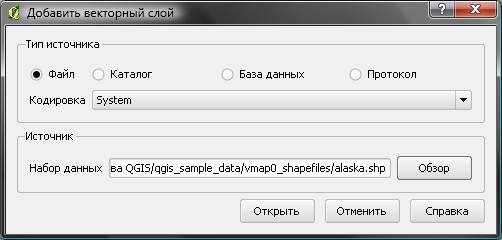
\includegraphics[clip=true, width=12cm]{addvectorlayerdialog}
   \caption{Диалог <<Добавить векторный слой>> \nixcaption}\label{fig:addvectorlayer}
\end{figure}

\begin{figure}[ht]
   \centering
   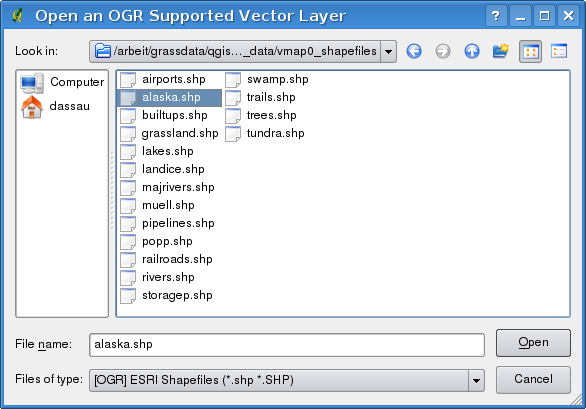
\includegraphics[clip=true, width=12cm]{shapefileopendialog}
   \caption{Диалог <<Открыть OGR-совместимый векторный слой>> \nixcaption}\label{fig:openshapefile}
\end{figure}

\begin{figure}[ht]
   \centering
   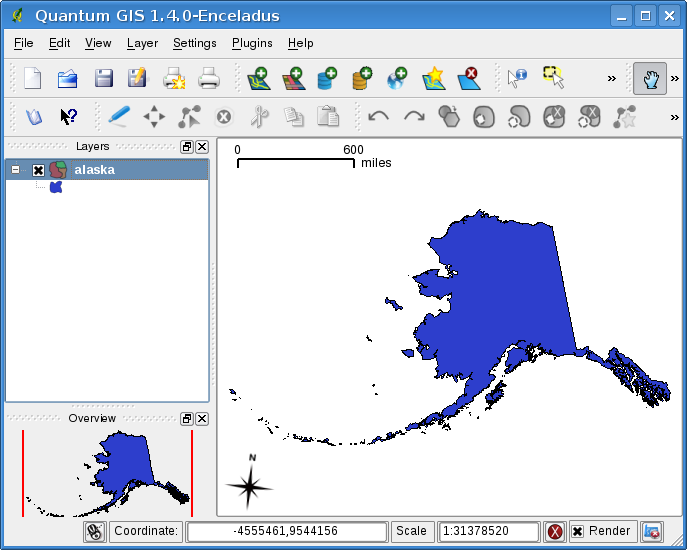
\includegraphics[clip=true, width=12cm]{shapefileloaded}
   \caption{\qg с загруженным shape-файлом Аляски \nixcaption}\label{fig:loadedshapefile}
\end{figure}

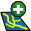
\includegraphics[width=0.7cm]{mActionAddNonDbLayer} Чтобы добавить shape-файл
надо использовать кнопку \toolbtntwo{mActionAddNonDbLayer}{Добавить векторный слой}
\index{shapefile!loading} или сочетание клавиш \keystroke{Ctrl+Shift+V}.
Появится новое диалоговое окно (см. Рисунок~\ref{fig:addvectorlayer}).

В разделе <<Тип источника>> надо отметить \radiobuttonon{{}Файл}. Нажмите
кнопку \button{Обзор}. При этом появится стандартный диалог открытия файла
(см. Рисунок~\ref{fig:openshapefile}) который позволяет выбрать и добавть
нужный shape-файл или другой поддерживаемый источник данных. Выпадающее меню
фильтра типов файлов \selectstring{{}Тип файлов}\ldots позволяет фильтровать
файлы с форматами, поддерживаемыми библиотекой OGR.

Для выбранного shape-файла можно указать кодировку атрибутивных данных.

Выбор shape-файла из списка и нажатие кнопки \button{Открыть} загружает
файл в \qg. Рисунок~\ref{fig:loadedshapefile} демонстрирует \qg после
открытия файла \filename{alaska.shp}.


\begin{Tip}\caption{\textsc{Цвет слоя}}
Каждому вновь добавленному к карте слою присваивается случайный цвет.
Если было открыто несколько слоёв, каждому присваивается свой цвет,
отличный от других.
\end{Tip}

Для навигации по открытому shape-файлу можно воспользоваться инструментами
с панели навигации. Чтобы изменить символику слоя, следует открыть диалог
\dialog{Свойства слоя} двойным щелчком мыши на названии слоя или щёлкнув
правой кнопкой мыши на названии слоя в легенде и выбрав пункт
\dropmenuopt{Свойства} из всплывающего меню. Дополнительную информацию
о символике векторных слоёв можно найти в Разделе~\ref{sec:symbology}.

\begin{Tip}\caption{\textsc{Добавление слоя или проекта со внешнего носителя в OS X}}
В OS X подключённые внешние устройства не появляются после выбора <<Файл>> \arrow
<<Открыть проект>>. Мы работаем над разрешением этой проблемы в диалогах
открытия и сохранения в OS X. В качестве временного решения можно напечатать
<</Volumes>> в поле имени файла и нажать Ввод. После этого можно указать путь
ко внешним носителям и сетевым дискам.
\end{Tip}

\subsection{Улучшение производительности}

Для увеличения производительности при отрисовке shape-файла можно создать
пространственный индекс. Пространственный индекс \index{spatial index!shapefiles}
улучшает скорость отрисовки как при изменении масштаба, так и при
панорамировании (перемещении слоя в каком-либо направлении без изменения
масштаба). Файл пространственного индекса, используемого \qg имеет
расширение \filename{.qix}.

Чтобы создать индекс, необходимо:

\begin{itemize}[label=--]
\item Открыть shape-файл.
\item Открыть диалог \dialog{Свойства соля} двойным щелчком по имени
shape-файла в легенде или правым щелчком по нему же и выбором
\dropmenuopt{Свойства} во всплывающем меню.
\item Во вкладке \tab{Общие} нажмите кнопку \button{Создать пространственный индекс}.
\end{itemize}

\subsection{Добавление на карту слоя MapInfo}
\index{vector layers!MapInfo}

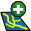
\includegraphics[width=0.7cm]{mActionAddNonDbLayer} Чтобы открыть слой
MapInfo, нажмите кнопку \toolbtntwo{mActionAddNonDbLayer}{Добавить
векторный слой} на панели инструментов или воспользуйтесь комбинацией
\keystroke{Ctrl+Shift+V}, измените \\
\selectstring{{}Тип файлов}{[OGR] MapInfo (*.mif*.tab *.MIF *.TAB)}
и выберете нужный файл.

\subsection{Добавление на карту покрытия ArcInfo}
\index{vector layers!ArcInfo Binary Coverage}

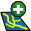
\includegraphics[width=0.7cm]{mActionAddNonDbLayer} Чтобы открыть покрытие ArcInfo
в двоичном формате, нажмите на кнопку
\toolbtntwo{mActionAddNonDbLayer}{Добавить векторный слой} на панели
инструментов или воспользуйтесь комбинацией клавиш \keystroke{Ctrl+Shift+V},
чтобы открыть диалог \dialog{Добавить векторный слой}. В качестве
<<Типа источника>> выберите \radiobuttonon{{}Каталог}. Выберите \\
\selectstring{{}Тип файлов}{Arc/Info Binary Coverage}. Укажите путь к каталогу
с файлами покрытия.

Аналогично добавляются векторные слои UK National Transfer Format и
TIGER Format Бюро переписи населения США (US Census Bureau).

\section{Слои PostGIS}
\index{vector layers!PostGIS|see{PostGIS}}
\index{PostGIS!layers}
\label{label_postgis}

Слои PostGIS хранятся в базе данных PostgreSQL. Преимуществами PostGIS
являются пространственное индексирование и широкие возможности
фильтрации и построения запросов. При использовании PostGIS, такие функции,
как выбор и идентификация работают более точно, чем при использовании
OGR-совместимых слоёв.
% оригинал предыдущей строчки (не уверен в корректности "идентификации"):
% vector functions such as select and identify work more accurately than
% with OGR layers in \qg.

Для использования слоёв PostGIS необходимо:\index{PostgreSQL!loading layers}

\begin{itemize}[label=--]
\item Задать настройки подключения \qg к базе данных PostgreSQL (если они
ещё не заданы).\index{PostgreSQL!connection}
\item Соединиться с базой данных.
\item Выбрать нужный слой.
\item По желанию задать SQL-запрос \usertext{where}, определяющий конкретные
объекты из слоя, которые необходимо загрузить.
\item Добавить слой.
\end{itemize}

\subsection{Настройка подключения к базе данных PostGIS (PostgreSQL)}\index{PostgreSQL!connection}\label{sec:postgis_stored}

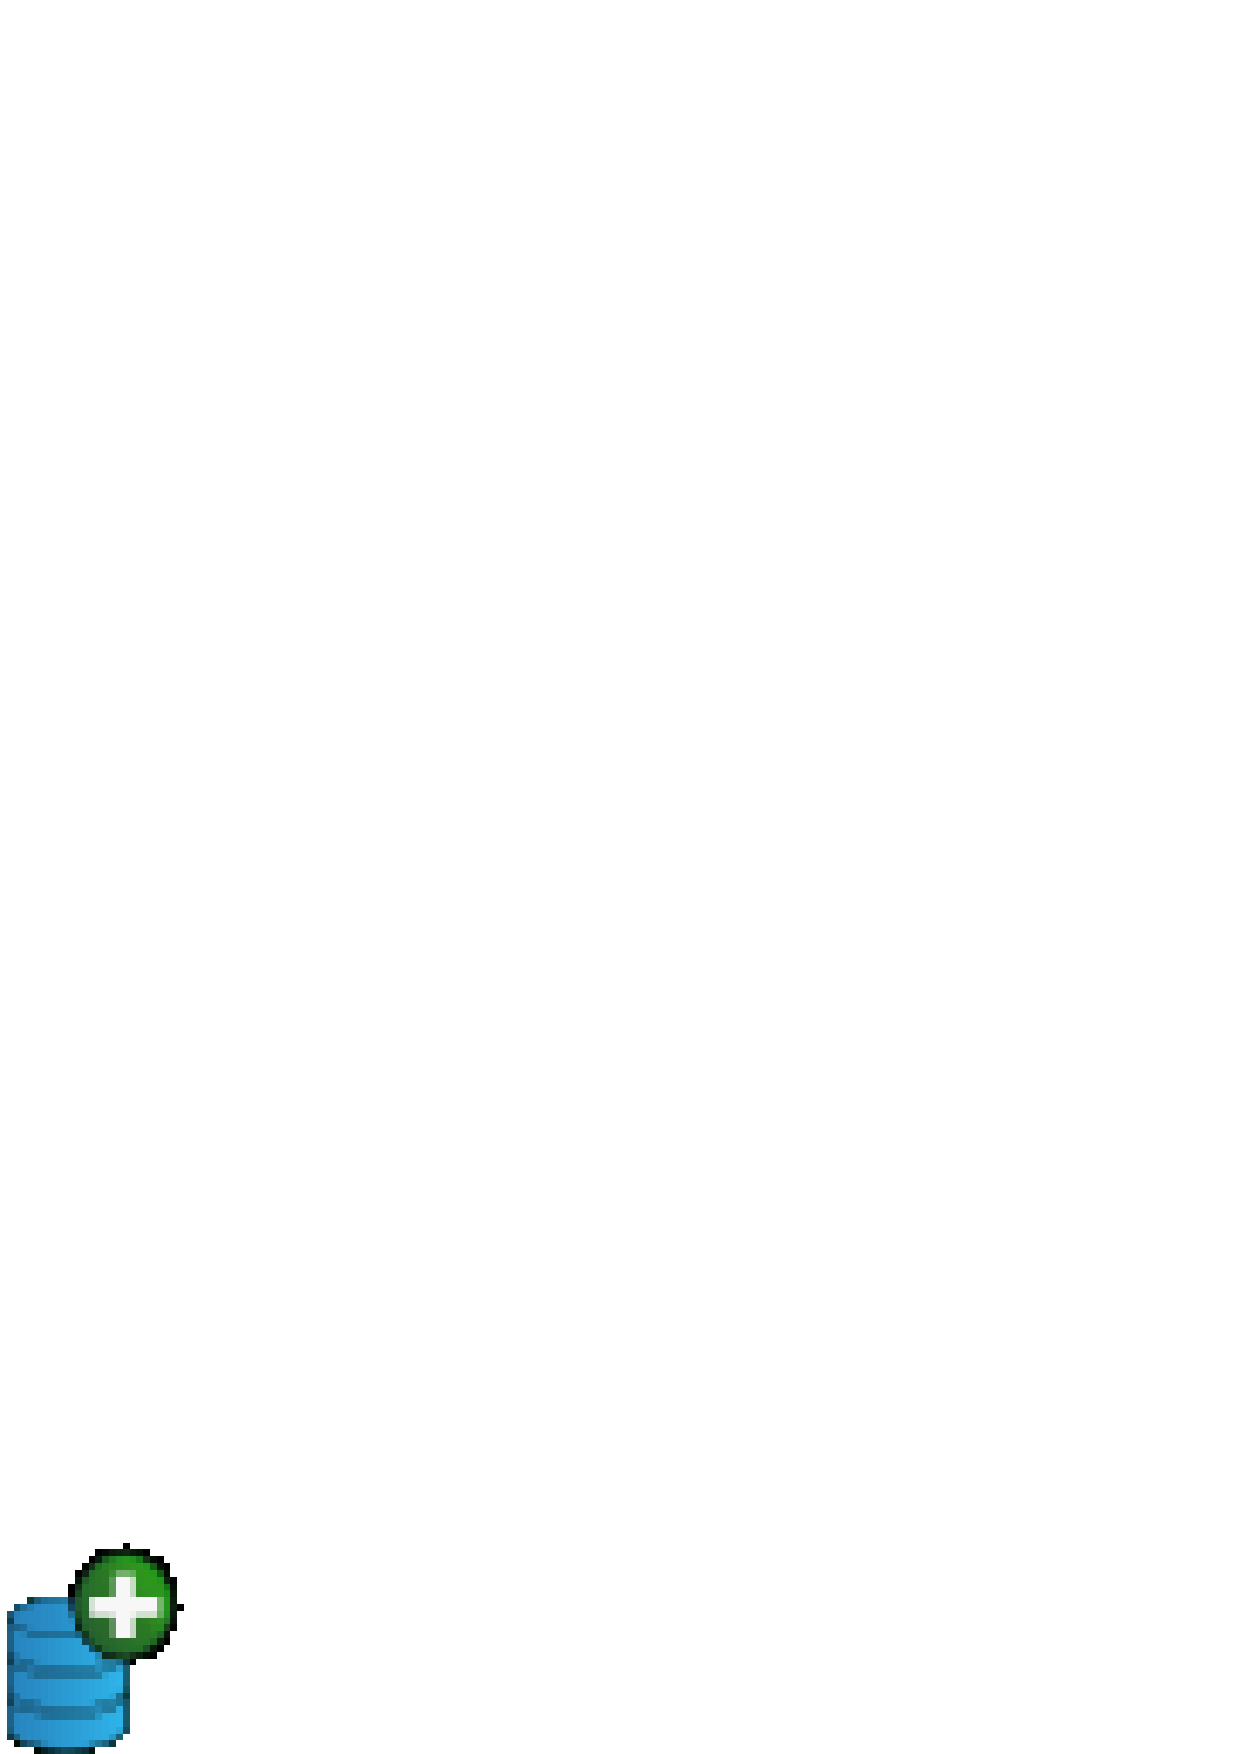
\includegraphics[width=0.7cm]{mActionAddLayer} При первом использовании
данных PostGIS, необходимых настроить подключение к базе данных PostgreSQL
содержащей нужную информацию. Нажмите на кнопку
\toolbtntwo{mActionAddLayer}{Добавить слой PostGIS} на панели инструментов
или выберите опцию \dropmenuopttwo{mActionAddLayer}{Добавить слой PostGIS...}
из меню \mainmenuopt{Слой}, также можно воспользоваться комбинацией клавиш
\keystroke{Ctrl+Shift+D}. Ещё один вариант "--- открыть диалог
\dialog{Добавить векторный слой} и выбрать \radiobuttonon{{}База данных}.
Появится диалог \dialog{Добавить таблицы PostGIS}. Для получения доступа
к менеджеру соединений\index{PostgreSQL!connection manager}, нажмите кнопку
\button{Создать}. \\
Появится диалог \dialog{Новое PostGIS соединение}. Параметры соединения
описаны в таблице~\ref{tab:postgis_connection_parms}.

\begin{table}[ht]\index{PostgreSQL!connection parameters}
\centering
\caption{Параметры подключения PostGIS}\label{tab:postgis_connection_parms}\medskip
 \begin{tabular}{|l|p{5in}|}
\hline Имя & Имя для данного соединения. Может совпадать с именем\textsl{Базы данных}.
\\
\hline Узел \index{PostgreSQL!host}
& Имя узла на котором хранится база данных. Имя узла должно быть допустимым:
таким какие используют для сетевого доступа или для пинга узла. Если база
данных находится на том же компьютере, что и \qg, просто введите здесь
<<localhost>>. \\
\hline База данных \index{PostgreSQL!database} & Имя базы данных. \\
\hline Порт \index{PostgreSQL!port}& Номер порта, который <<слушает>>
сервер базы данных PostgreSQL. По умолчанию используется порт 5432.\\
\hline SSL-режим \index{PostgreSQL!sslmode}& Настройка SSL-режима работы
с сервером. Можно выбрать:
\begin {itemize}
\item запретить: использовать только не зашифрованное SSL-соединение;
\item разрешить: будет произведена попытка установки не SSL-соединения,
если она не удастся, будет использовано SSL-соединение;
\item предпочитать (по умолчанию): будет произведена попытка установки
SSL-соединения, если она не удастся, будет использовано не SSL-соединение;
\item требовать: использовать только SSL-соединение.
\end {itemize}
Следует отметить, что значительного прироста скорости рендеринга слоя PostGIS
можно достигнуть путём отключения SSL в менеджере соединений. \\
\hline Пользователь \index{PostgreSQL!username}& Имя пользователя, которое
используется для доступа к базе данных. \\
\hline Пароль \index{PostgreSQL!password}& Пароль используемый вместе с
\textsl{именем пользователя} для подключения к базе данных.\\
\hline
\end{tabular}
\end{table}

Есть возможность выбрать дополнительные параметры:

\begin{itemize}[label=--]
\item \checkbox{Сохранить пользователя}
\item \checkbox{Сохранить пароль}
\item \checkbox{Искать только в таблице <<geometry\_columns>>}
\item \checkbox{Искать только в схеме <<public>>}
\item \checkbox{Использовать расчётные метаданные таблицы}
\end{itemize}

Когда параметры установлены, можно проверить соединение путём нажатия
на кнопку \button{Проверить соединение} button\index{PostgreSQL!connection!testing}.

\begin{Tip}\caption{\textsc{\qg Пользовательские настройки и безопасность}}
\index{settings}\index{security}
В зависимости от используемой операционной системы \qg хранит
пользовательские настройки: в Домашней папке на \nix системах
\filename{.\qg/}; в реестре, если используется \win. В зависимости
от используемой операционной системы и настроек компьютера, хранение пароля
в настройках \qg может создавать угрозу безопасности.
\end{Tip}

\subsection{Добавление соля PostGIS к карте}\index{PostgreSQL!loading layers}

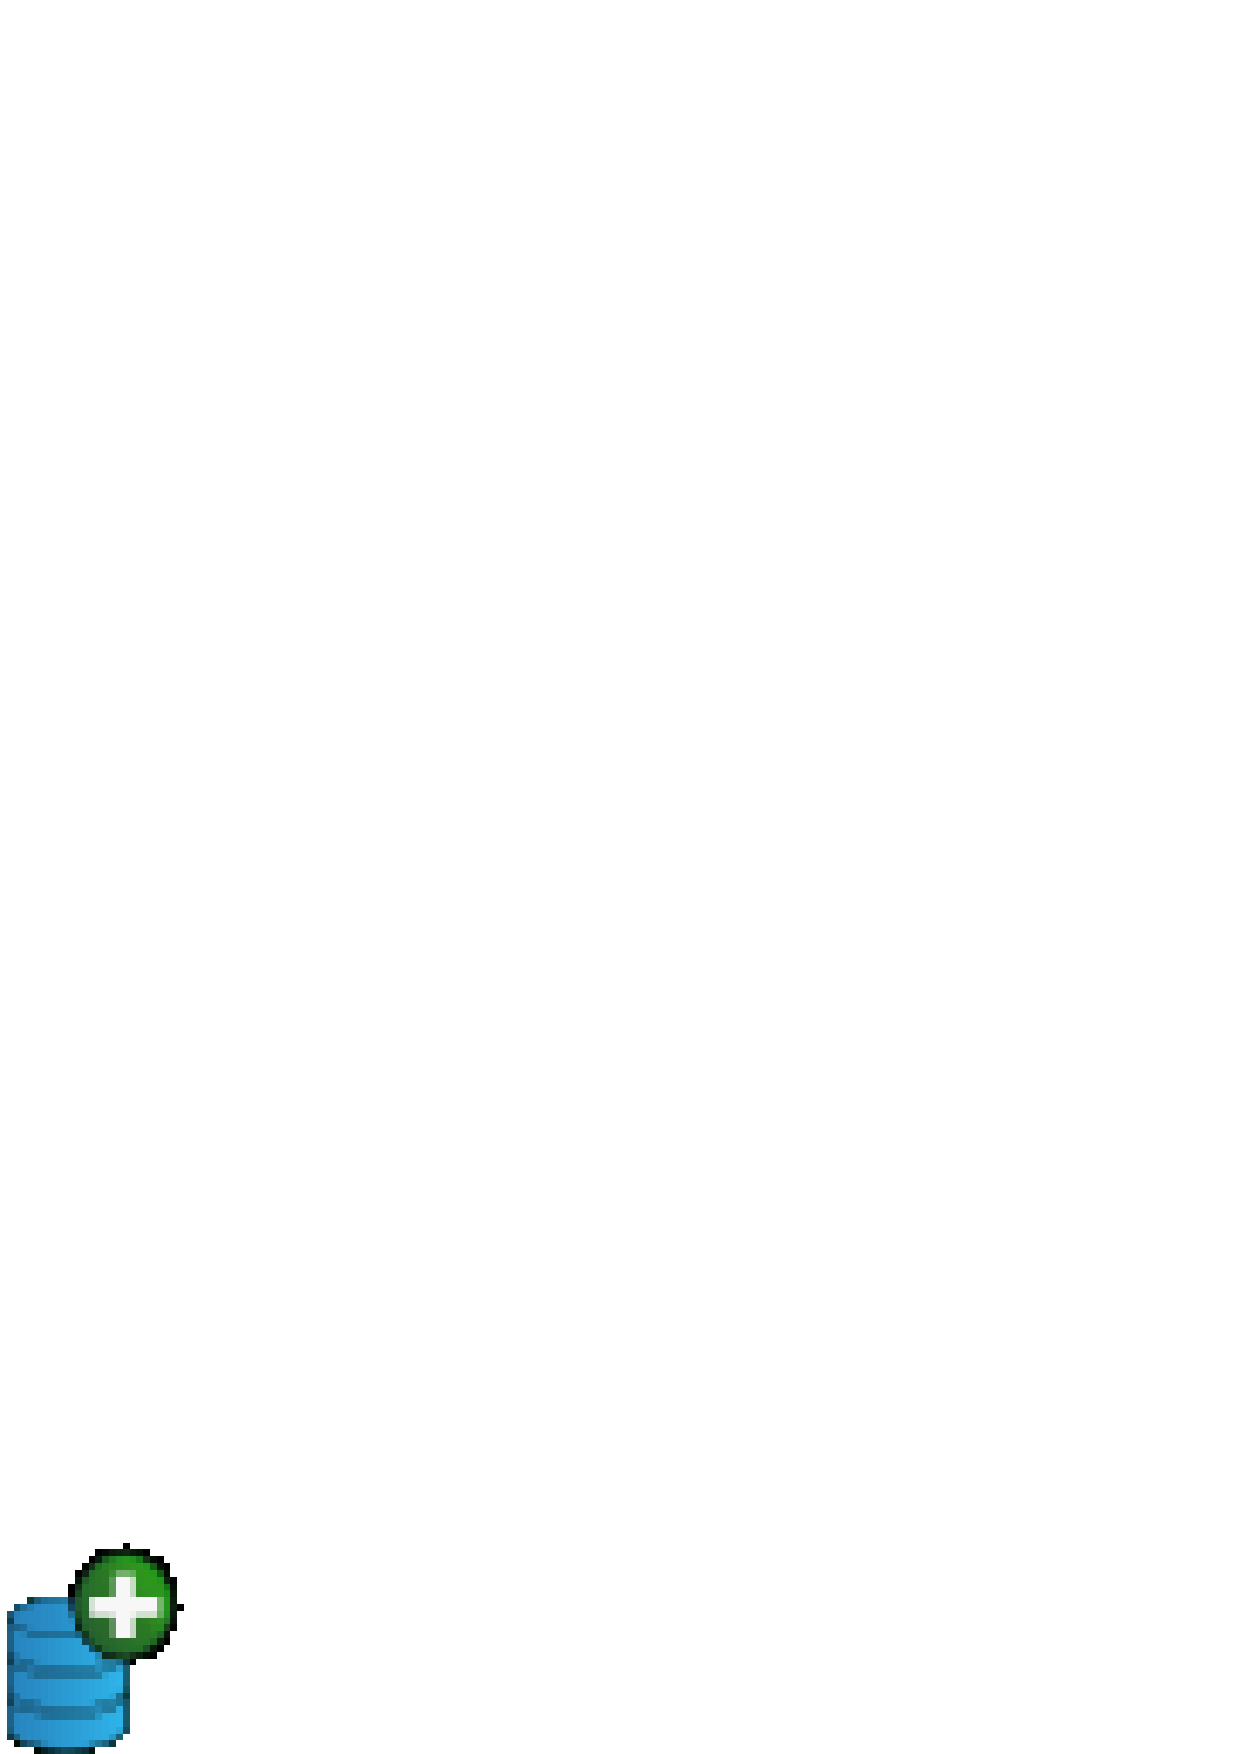
\includegraphics[width=0.7cm]{mActionAddLayer} Когда создано одно или
более соединение, можно добавлять слои из PostgreSQL. Естественно, в базе
данных PostgreSQL должна содержаться информация. Смотри
Раздел~\ref{sec:loading_postgis_data}, в котором обсуждается импорт данных
в базу данных.

Для открытия слоя PostGIS, проделайте следующие шаги:

\begin{itemize}[label=--]
\item Если диалог \dialog{Add PostGIS Table(s)} ещё не открыт, нажмите
кнопку \toolbtntwo{mActionAddLayer}{Добавить слой PostGIS} на панели
инструментов.
\item Выберите соединение из выпадающего списка и нажмите кнопку
\button{Подключиться}.
\item Найдите слой, который желаете добить в список доступных слоёв.
\item Щёлкните по нему, чтобы выбрать. Можно выбрать несколько слоёв,
если нажать и удерживать клавишу \keystroke{Shift}. В
Разделе~\ref{sec:query_builder} можно найти информацию об использовании
<<Конструктора запросов>> при работе с PostgreSQL.
\item Нажмите кнопку \button{Добавить} чтобы добавить слой к карте.
\end{itemize}

\begin{Tip}\caption{\textsc{Слои PostGIS}}
Обычно слои PostGIS определяются наличием записей в таблице
geometry\_columns. Начиная с версии \OLD % should be 0.9.0
, \qg может загружать слои, которые не имеют записей в таблице
geometry\_columns. Это касается таблиц и <<представлений>>. % представление - view
Задание пространственных представлений "--- мощное средство визуализации данных.
В руководстве пользователя PostgreSQL можно найти дополнительную информацию
по созданию представлений.
\end{Tip}

\subsection{Некоторые детали работы со слоями PostgreSQL}
\label{sec:postgis_details}
\index{PostgreSQL!layer details}

Этот раздел содержит некоторый подробности доступа к слоям PostgreSQL в \qg.
Обычно \qg обеспечивает доступ к списку таблиц базы данных, которые можно
добавить к карте и открывает их по запросу. Однако, если возникают трудности
с открытием таблиц PostgreSQL в \qg, следующая информация может помочь
понять сообщения \qg и подсказать способы изменения способа определения
таблицы или представления PostgreSQL, чтобы позволить \qg загрузить их.
% "изменения способа определение таблицы или представления" - "change PostgreSQL table or view defenition"

\qg требует наличия колонки в слое PostgreSQL, которая бы служила уникальным
идентификатором (ключом) слоя. Для таблиц это обычно означает, что они должны
иметь первичный ключ, или колонку с уникальными значениями строк в ней.
% оригинал - or a column with a unique constraint on it.
В \qg, эта колонка должна содержать значения типа int4 (целое число размером
4 байта). Альтернативный способ "--- использование колонки <<ctid>> в качестве
первичного ключа. Если в таблице отсутствуют колонки, указанные выше, то
вместо них будет использоваться колонка <<oid>>. Индексирование колонок позволит
повысить производительность (заметьте, что первичные ключи в PostgreSQL
индексируются автоматически).

Если слой PostgreSQL является представлением, к нему предъявляются те же
требования, что были описаны выше, но представления не имеют первичных
ключей или колонок с уникальными значениями. В этом случае \qg попытается
самостоятельно найти колонку в представлении, являющуюся производной от
колонки, удовлетворяющей необходимым условиям. % оригинал - derived from a suitable table column.
Это достигается посредством разбора SQL-опеределения представления % It does this by parsing the view definition SQL.
Однако, есть элементы SQL, игнорируемые \qg, например, использование
псевдонимов таблиц и колонок, создаваемых SQL-запросами.

Если невозможно найти подходящую колонку, \qg не откроет слой. В таком
случае следует изменить представление таким образом, чтобы оно содержало
требуемую колонку (тип int4 и либо являющуюся первичным ключом, либо
содержащую уникальные значения, желательно, индексированную).

%%FIXME: Add missing information
%% When dealing with views, \qg parses the view definition and

\subsection{Импорт данных в PostgreSQL}\label{sec:loading_postgis_data}
\index{PostGIS!SPIT!importing data}

\minisec{shp2pgsql}
Существует несколько способов импорта данных в базу данных PostgreSQL. PostGIS
поставляется с утилитой \filename{shp2pgsql}, которую можно использовать для
импорта shape-файлов в базу данных PostGIS. Например для импорта shape-файла
\filename{lakes.shp} в базу данных PostgreSQL, называющуюся
\usertext{gis\_data}, воспользуйтесь следующей командой:

\begin{verbatim}
  shp2pgsql -s 2964 lakes.shp lakes_new | psql gis_data
\end{verbatim}

При этом будет создан новый слой под названием \usertext{lakes\_new} в
базе данных \usertext{gis\_data}. Новый слой будет иметь идентификатор
системы координат (SRID) 2964. более подробную информацию о системах координат
и проекциях можно найти в Разделе~\ref{label_projections}
\begin{Tip}
\caption{\textsc{Экспорт наборов данных из PostGIS}\index{PostGIS!Exporting}}
Наряду с инструментом для импорта \filename{shp2pgsql} существует инструмент
для экспорта наборов данных PostGIS в shape-файл: \filename{pgsql2shp}.
Он также входит в поставку PostGIS.
\end{Tip}

\minisec{Модуль SPIT}

\includegraphics[width=0.7cm]{spiticon} \qg включает в себя модуль
SPIT (Shapefile to PostGIS Import Tool "--- инструмент импорта shape-файлов
в PostGIS)\index{PostGIS!SPIT}. SPIT способен осуществлять одновременный
импорт нескольких shape-файлов и поддерживает схемы баз данных. Для
использования SPIT, откройте <<Менеджер управления модулями>> \qg в меню
\mainmenuopt{Модули} и выберите пункт <<Управление модулями>>, поставьте
галочку напротив \checkbox{SPIT} и нажмите кнопку \button{OK}. Иконка
модуля SPIT появится на панели инструментов\index{PostGIS!SPIT!loading}.

Для импорта shape-файла нажмите на иконку \toolbtntwo{spiticon}{SPIT}
на панели инструментов. \\
Откроется диалог \dialog{SPIT - инструмент импорта shape-файлов в PostGIS}.
Выберите базу данных PostGIS с которой необходимо установит соединение и
нажмите кнопку \button{Подключиться}. Теперь можно добавить файлы в
очередь, нажимая кнопку \button{добавить}. Для запуска обработки файлов,
нажмите кнопку \button{OK}. Прогресс импорта, так же как и любые ошибки
или предупреждения будет показан после обработки каждого из shape-файлов.

\begin{Tip}\caption{\textsc{Импорт shape-файлов, содержащих
слова, зарезервированные PostgreSQL}}\index{PostGIS!SPIT!reserved words}
Если shape-файл, добавленный в очередь, содержит имена полей, зарезервированные
базой данных PostgreSQL, появится диалог, сообщающий статус каждого поля.
Можно изменить имена этих (и других) полей\index{PostGIS!SPIT!editing field names}
перед импортом. Попытки импорта shape-файла с именами полей, зарезервированными
PostgreSQL обречены на провал.
\end{Tip}

\minisec{ogr2ogr}
Кроме \filename{shp2pgsql} и \filename{SPIT} есть ещё один инструмент
импорта пространственной информации в PostGIS: \filename{ogr2ogr}, который
является частью установки GDAL. Для импорта shape-файла в PostGIS проделайте
следующее:
\begin{verbatim}
  ogr2ogr -f "PostgreSQL" PG:"dbname=postgis host=myhost.de user=postgres \
  password=topsecret" alaska.shp
\end{verbatim}

Эта команда импортирует файл \filename{alaska.shp} в базу данных PostGIS
\usertext{postgis} на сервере \server{myhost.de} используя в качестве
имени пользователя базы данных "--- \usertext{postgres},
с паролем "--- \usertext{topsecret}.

Заметьте, что для работы с PostGIS в OGR должна быть включена поддержка
PostgreSQL. Проверить её наличие можно с помощью команды
\begin{verbatim}
ogrinfo --formats | grep -i post
\end{verbatim}

Те, кто предпочитают использовать команду PostgreSQL \filename{COPY}
вместо метода \filename{INSERT INTO}, используемого по умолчанию, могут
экспортировать следующие переменные среды (по крайней мере доступно на
\nix и \\ \osx):
\begin{verbatim}
  export PG_USE_COPY=YES
\end{verbatim}

\filename{ogr2ogr} не создаёт пространственный индекс, как это делает
\filename{shp2pgsl}. Его необходимо создать вручную, используя SQL-команду
\filename{CREATE INDEX} после экспорта (смотри описание в следующем
Разделе~\ref{label_improve}).

\subsection{Повышение производительности} \label{label_improve}

Получение данных, находящихся в базе данных PostgreSQL может серьёзно
снижать производительность, особенно при работе через сеть. Производительность
при отрисовке можно улучшить путём создания пространственного индекса для
каждого слоя базы данных PostgreSQL \index{PostGIS!spatial index}.
PostGIS поддерживает создание \index{PostGIS!spatial index!GiST} GiST-индекса
(Generalized Search Tree) для ускорения пространственного поиска данных.

Ниже представлен порядок создания GiST\footnote{Информация о GiST-индексе
взята из документации к PostGIS, доступной на
\url{http://postgis.refractions.net}}-индекса:

\begin{verbatim}
    CREATE INDEX [indexname] ON [tablename]
      USING GIST ( [geometryfield] GIST_GEOMETRY_OPS );
\end{verbatim}

Заметьте, что для больших таблиц создание индекса может занять
продолжительное время. После создания индекса следует произвести
\usertext{VACUUM ANALYZE}. Дополнительную информацию можно найти в
документации к PostGIS \cite{PostGISweb}.

Приведём пример создания GiST-индекса:
\begin{verbatim}
gsherman@madison:~/current$ psql gis_data
Welcome to psql 8.3.0, the PostgreSQL interactive terminal.

Type:  \copyright for distribution terms
        \h for help with SQL commands
        \? for help with psql commands
        \g or terminate with semicolon to execute query
        \q to quit

gis_data=# CREATE INDEX sidx_alaska_lakes ON alaska_lakes
gis_data-# USING GIST (the_geom GIST_GEOMETRY_OPS);
CREATE INDEX
gis_data=# VACUUM ANALYZE alaska_lakes;
VACUUM
gis_data=# \q
gsherman@madison:~/current$
\end{verbatim}

\subsection{Векторные слои, пересекающие долготу 180$^\circ$}
\index{vector layers!crossing}

Многие ГИС испытывают трудности при работе с векторными картами в системе
координат широта/долгота (lat/lon), пересекающими долготу \degrees{180}.
При открытии таких карт в \qg, можно наблюдать две разнесённые на большое
удаление друг от друга части территории/акватории, которые на самом деле
представляют собой единое целое. На рисунке~\ref{fig:vector_not_wrapping}
едва заметные точки в левой части карты (архипелаг Чатем), должны
находиться внутри сетки, справа от главных островов (Северного и Южного)
Новой Зеландии.
% названия островов в оригинале мануала отсутствуют
% подумал, что имеет смысл сделать это уточнение, но если это лишнее - можно удалить

\begin{figure}[ht]
   \centering
   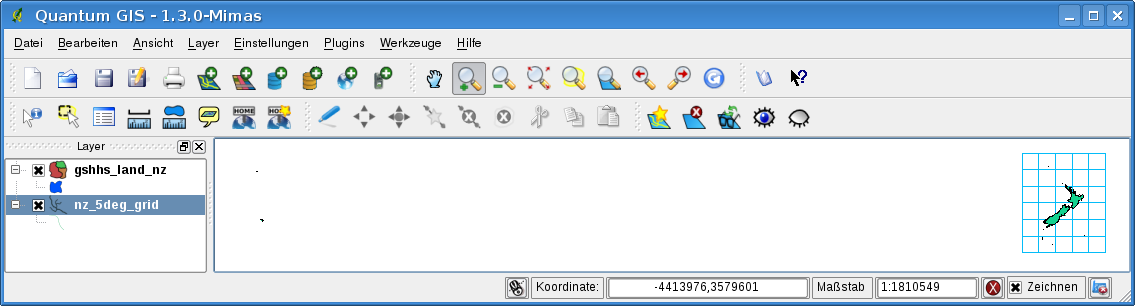
\includegraphics[clip=true, width=\textwidth]{vectorNotWrapping}
      \caption{Карта в системе координат широта/долгота, пересекающая долготу \degrees{180} \nixcaption}
   \label{fig:vector_not_wrapping}
\end{figure}

В качестве одного из вариантов решения проблемы можно трансформировать
значения координат долготы при помощи PostGIS и функции
\textbf{ST\textunderscore Shift\textunderscore Longitude}
\footnote{\url{http://postgis.refractions.net/documentation/manual-1.4/ST\_Shift\_Longitude.html}}.
Эта функция проверяет каждую точку (или узел) каждого объекта слоя, и,
если координаты долготы < \degrees{0}, добавляет \degrees{360} к значению.
На результирующей карте долгота объектов будет лежать в пределах
\degrees{0} -- \degrees{360} а сама карта будет отцентрирована по
\degrees{180} долготы.

\begin{figure}[ht]
   \centering
   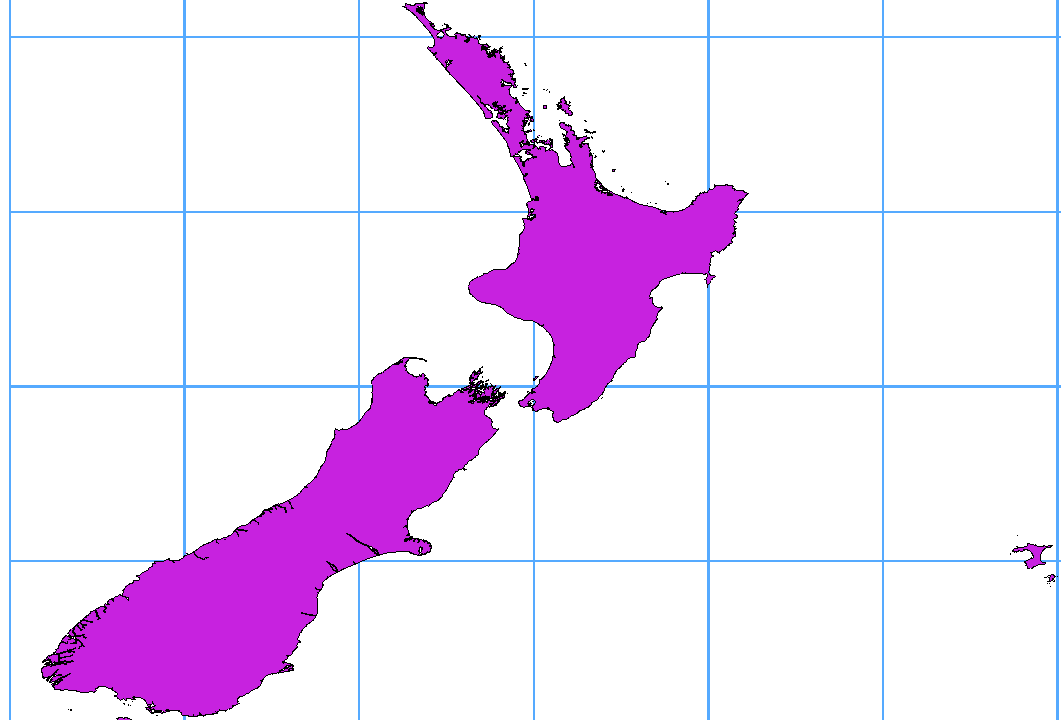
\includegraphics[clip=true, width=9cm]{vectorWrapping}
   \caption{Карта, пересекающая долготу \degrees{180}: после применения функции ST\textunderscore Shift\textunderscore Longitude \nixcaption}
\label{fig:vector_wrapping}
\end{figure}

\minisec{Использование}

\begin{itemize}[label=--]
\item Импортируем данные в PostGIS (\ref{sec:loading_postgis_data}) при помощи
модулей <<PostGIS Manager>> или <<SPIT>>
\item Используя командную строку PostGIS, выполните следующую команду
(в этом примере <<TABLE>> "--- имя вашей таблицы PostGIS): \\
\texttt{gis\_data=\# update TABLE set the\_geom=ST\_shift\_longitude(the\_geom);}
\item Если операция прошла успешна, появится подтверждение о количестве
объектов, информация о которых обновлена, после этого будет возможно добавить
объекты на карту и увидеть изменения (см. Рисунок~\ref{fig:vector_wrapping})
\end{itemize}

\section{Слои SpatiaLite}
\index{SpatiaLite layers!properties dialog}
\index{vector layers!SpatlaLIte|see{SpatiaLite}}
\index{SpatiaLite!layers}
\label{label_spatialite}

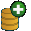
\includegraphics[width=0.7cm]{mActionAddSpatiaLiteLayer}
При первой загрузке слоёв из базы данных SpatiaLite database воспользуйтесь
кнопкой \\
\toolbtntwo{mActionAddSpatiaLiteLayer}{Добавить слой SpatiaLite}
на панели инструментов или пунктом
\dropmenuopttwo{mActionAddSpatiaLiteLayer}{Добавить слой SpatiaLite...}
меню \mainmenuopt{Слой}, либо комбинацией клавиш \keystroke{Сtrl+Shift+L}.
Появится окно, которое позволит соединиться с базой данных SpatiaLite,
которая уже была подключена к \qg ранее (её можно выбрать в выпадающем
меню), или же создать новое подключение. Для создания нового подключения
нажмите на кнопку \button{Создать} и используйте менеджер файлов, чтобы
указать путь к нужной базе данных (файлу с расширением \filename{.sqlite }).

\section{The Vector Properties Dialog}\label{sec:vectorprops}
\index{vector layers!properties dialog}

The \dialog{Layer Properties} dialog for a vector layer provides information
about the layer, symbology settings and labeling options. If your vector
layer has been loaded from a PostgreSQL/PostGIS datastore, you can also alter
the underlying SQL for the layer by invoking the \dialog{Query Builder}
dialog on the \tab{General} tab.
To access the \dialog{Layer Properties} dialog, double-click on a layer in
the legend or right-click on the layer and select \dropmenuopt{Properties}
from the popup menu.

\begin{figure}[ht]
   \centering
   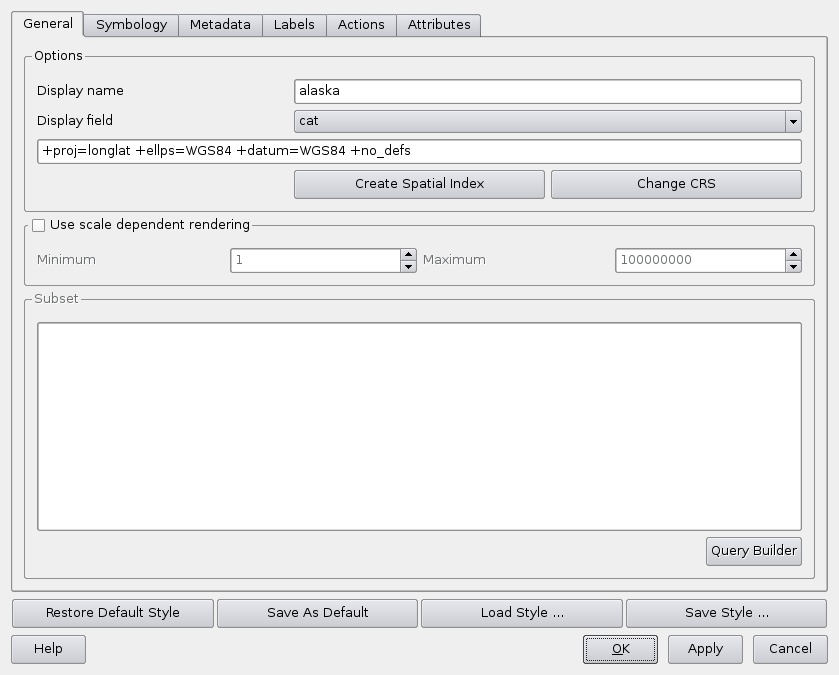
\includegraphics[clip=true, width=12cm]{vectorLayerSymbology}
   \caption{Vector Layer Properties Dialog \nixcaption}\label{fig:vector_symbology}
 \end{figure}

\subsection{Symbology Tab}\label{sec:symbology}
\index{vector layers!symbology}

\qg supports a number of symbology renderers to control how
vector features are displayed. Currently the following renderers
are available:

\begin{description}
    \item[Single symbol] - a single style is applied to every
    object in the layer.\index{vector layers!renderers!single symbol}
    \item[Graduated symbol] - objects within the layer are
    displayed with different symbols classified by the values of a
    particular field.\index{vector layers!renderers!graduated symbol}
    \item[Continuous color] - objects within the layer are
    displayed with a spread of colours classified by the numerical
    values within a specified field.\index{vector layers!renderers!continuous
color}
    \item[Unique value] - objects are classified by the unique
    values within a specified field with each value having a
    different symbol.\index{vector layers!renderers!unique value}
\end{description}

To change the symbology for a layer, simply double click on its legend
entry and the vector \dialog{Layer Properties} dialog will be
shown.\index{symbology!changing}

\begin{figure}[ht]
\centering
\caption{Symbolizing Options \nixcaption}
   \subfloat[Single symbol] {\label{subfig:single_symbol}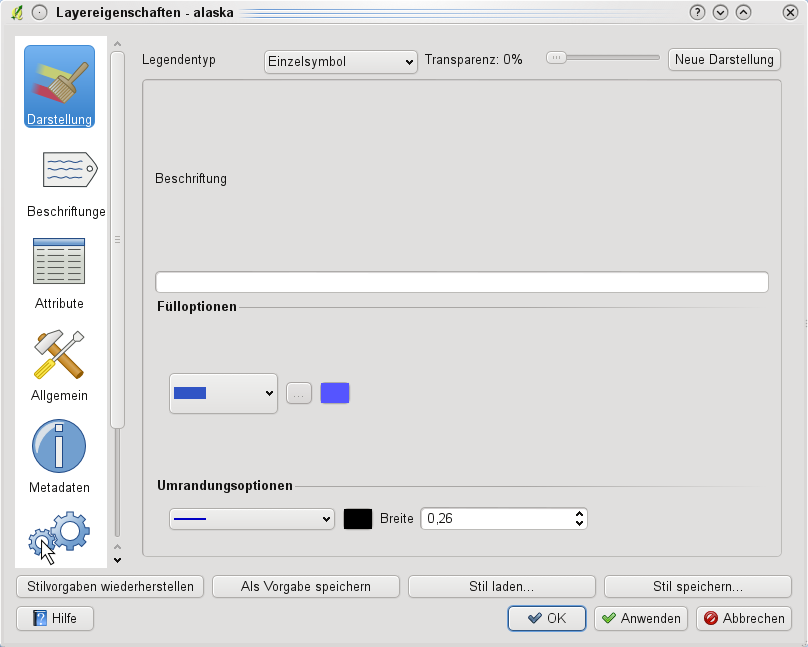
\includegraphics[clip=true, width=0.4\textwidth]{vectorClassifySingle}}
   \hspace{1cm}
   \subfloat[Graduated symbol] {\label{subfig:graduated_symbol}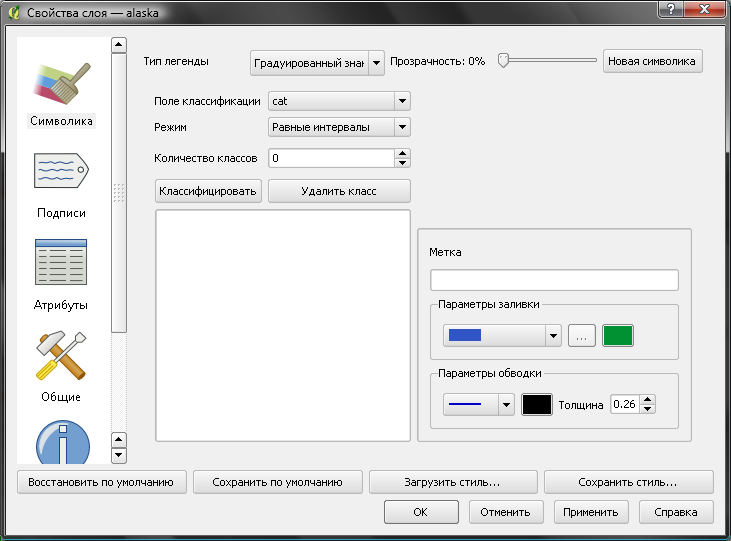
\includegraphics[clip=true, width=0.4\textwidth]{vectorClassifyGraduated}}
   \hspace{1cm}
   \subfloat[Continous color] {\label{subfig:cont_color}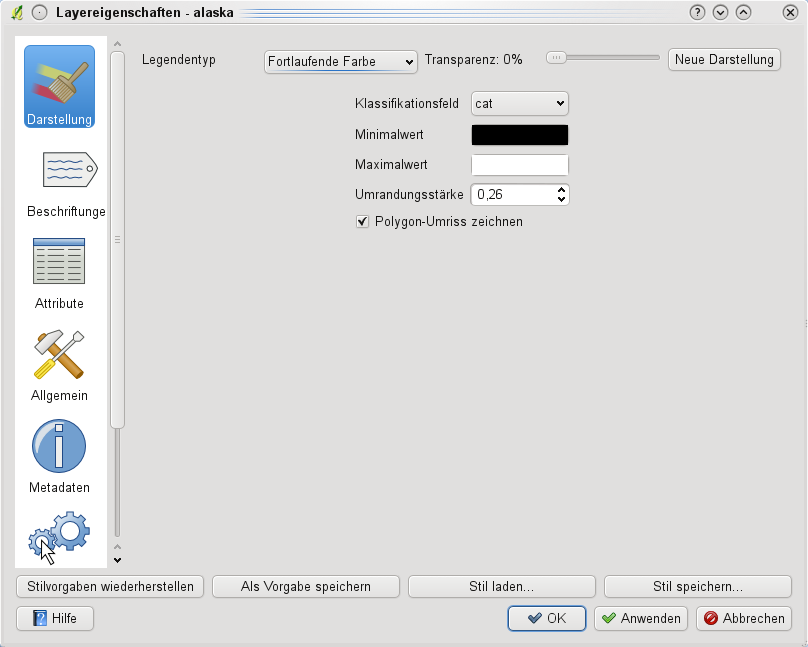
\includegraphics[clip=true, width=0.4\textwidth]{vectorClassifyContinous}}
   \hspace{1cm}
   \subfloat[Unique value] {\label{subfig:unique_val}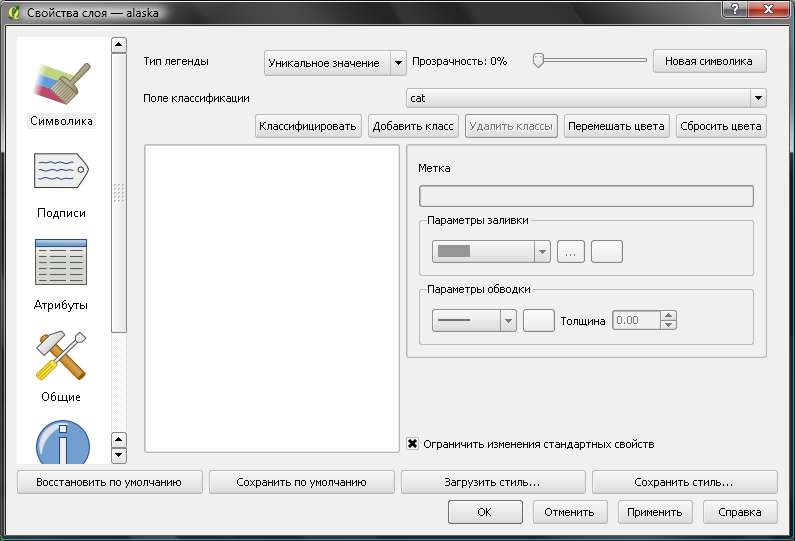
\includegraphics[clip=true, width=0.4\textwidth]{vectorClassifyUnique}}
\end{figure}

% FIXME: outdated
% Since \usertext{version v0.9} there is a function to use image files stored on
% your computer as fill pattern for vector layers.

\minisec{Style Options} \label{sec:style_options} \index{vector layers!styles}
Within this dialog you can style your vector layer. Depending on the selected
rendering option you have the possibility to also classify your mapfeatures.

At least the following styling options apply for nearly all renderers:
\begin{description}
\item[Fill options]
\begin{description}
 \item[Fill style] - Style for filling. Beside the given brushes you can
 select \selectstring{Fill style}{? Texture} and click the \browsebutton
 button for selecting your own texture file. Currently the fileformats
 \filename{*.jpeg, *.xpm, and *.png} are supported.
 \item[Fill color] - fill-color of your features.
\end{description}
\item[Outline options]
\begin{description}
 \item[Outline style] - pen-style for your outline of your feature. You can
 also set this to 'no pen'.
 \item[Outline color] - color of the ouline of your feature.
 \item[Outline width] - width of your features.
\end{description}
\end{description}

Once you have styled your layer you also could save your layer-style to a
separate file (with \filename{*.qml}-ending).
To do this, use the button \button{Save Style \ldots}. No need to say that
\button{Load Style \ldots} loads your saved layer-style-file.

If you wish to always use a particular style whenever the layer is loaded,
use the \button{Save As Default} button to make your style the default. Also,
if you make changes to the style that you are not happy with, use the \button{Restore
Default Style} button to revert to your default style.

\minisec{Vector transparency} \label{sec:vect_transparency}
\index{vector layers!transparency}

\qg allows to set a transparency for every vector layer. This can be done with
the slider \\
\slider{Transparency} inside the \tab{symbology} tab (see
fig. \ref{subfig:single_symbol}). This is very useful for overlaying several
vector layers.

\subsection{New Generation Symbology}

Since \qg 1.4.0  a new symbology was integrated in parallel with the symbology
described above. This new generation symbology provides a variety of improvements and
new features and will replace the current symbology in one of the upcoming releases.
To switch to the new symbolgy you currently have to click on the \button{New symbology} button in the \tab{General} tab of the \dialog{Layer Properties} dialog. You can
also make the New symobolgy the default, activating \checkbox{Use new generation symbology for rendering} in the \tab{Rendering \& SVG} tab under the \mainmenuopt{Settings} > \dropmenuopt{Options} menu.

\minisec{Understanding the new generation symbology}

There are three types of symbols: marker symbols (for points), line symbols and
fill symbols (for polygons). Symbols can consist of one or more symbol layers. It
is possible to define the color of a symbol and this color is then defined for all
symbol layers. Some layers may have the color locked - for those the color can not
be altered. This is useful when you define the color of a multilayer symbol.
Similarly, it is possible to define the width for line symbols, as well as size and
angle for marker symbols.

\minisec{Available symbol layer types}

\begin{itemize}[label=--]
\item \textbf{Simple marker}: Rendering with one of hardcoded markers.
\item \textbf{Simple line}: Usual rendering of a line (with specified
width, color and pen style).
\item \textbf{Simple fill}: Usual rendering of a polygon (with defined
fill color, fill pattern and outline).
\item \textbf{SVG marker}: Rendering with a SVG picture.
\item \textbf{Marker line}: A line rendered by repeating a marker symbol.
\end{itemize}

\minisec{Color ramps}

Color ramps are used to define a range of colors that can be used during
the creation of renderers. The symbol's color will be set from the color ramp.

There are three types of color ramps:

\begin{itemize}[label=--]
\item \textbf{Gradient}: Linear gradient from one color to some other.
\item \textbf{Random}: Randomly generated colors from a specified area of
color space.
\item \textbf{ColorBrewer}: Create color area from a color shema and a defined
number of color classes.
\end{itemize}

Color ramps can be defined in the \dialog{Style Manager} dialog (see Section
\ref{subsec:stylemanager}) by selecting \\
\selectstring{Style item type:}{Color ramp} as style element type from the drop-down list, clicking on \button{Add item} button and then choosing a color ramp type.

\minisec{Styles}

A style groups a set of various symbols and color ramps. You can define your
prefered or frequently used symbols, and can use it without having to recreate
it everytime. Style items (symbols and color ramps) have always a name by which
they can be queried from the style. There is one default style in \qg (modifiable)
and the user can add further styles.

\minisec{Renderers}

The renderer is responsible for drawing a feature together with the correct
symbol. There are three types of renderers: single symbol, categorized (called
unique color in the old symbology), and graduated. There is no continuous color
renderer, because it is in fact only a special case of the graduated renderer.
The categorized and graduated renderer can be created by specifying a symbol
and a color ramp - they will set the colors for symbols appropriately.

\subsection{Working with the New Generation Symbology}

First you have to enable the new generation symbology clicking on the
\button{New symbology} button in the \tab{Symbology} tab of the
\dialog{Layer Properties} dialog. The new dialog allows to choose one of the
three renderers: single symbol, categorized and graduated. Depending on the
chosen renderer, the symbology tab provides different settings and options, that
will be described in the following sections.

\minisec{Single Symbol Renderer}

The Single Symbol Renderer is used to render all features of the layer using a
single user-defined symbol. The properties, that can be adjusted in the
Symbology tab, depend partially on the type of the layer, but all types share
the following structure. In the top left part of the tab, there is a preview of
the current symbol to be rendered. In the bottom part of the tab, there is a
list of symbols already defined for the current style, prepared to be used via
selecting them from the list. The current symbol can be modified using the
\button{Properties} button, which opens a \dialog{Symbol Properties} dialog, or
the \button{Set Color} button, which opens an ordinary \dialog{Color} dialog.
After having done any needed changes, the symbol can be added to the list of
current style symbols (using the \button{Add to style} button) and then easily
be used in the future.

\begin{figure}[ht]
\centering
   \subfloat[Single symbol point properties] {\label{subfig:singleNG1}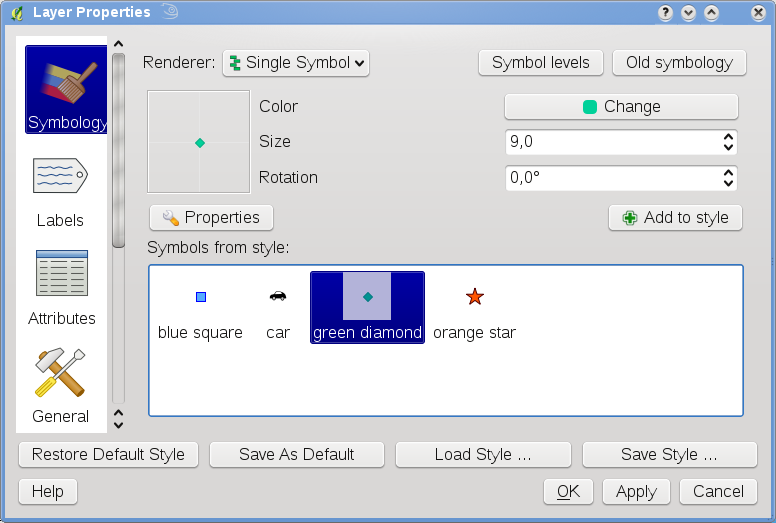
\includegraphics[clip=true, width=0.3\textwidth]{singlesymbol_ng_point}}
   \hspace{1cm}
   \subfloat[Single symbol line properties] {\label{subfig:singleNG2}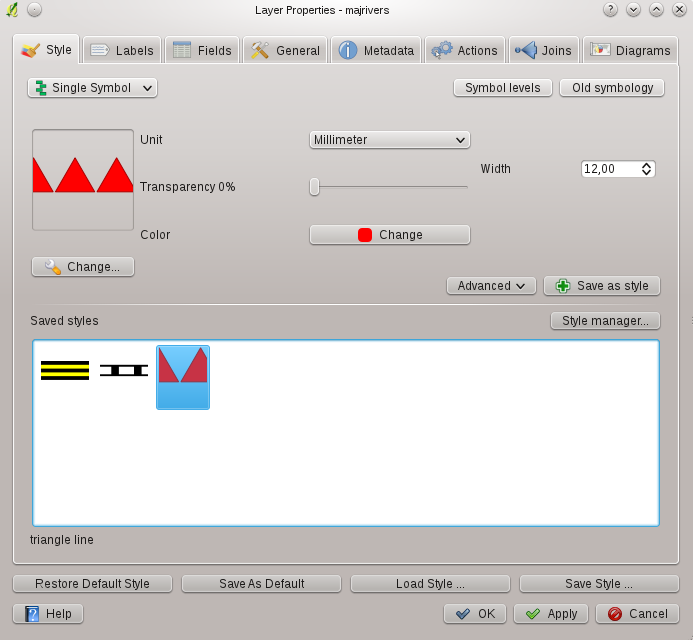
\includegraphics[clip=true, width=0.3\textwidth]{singlesymbol_ng_line}}
   \hspace{1cm}
   \subfloat[Single symbol area properties] {\label{subfig:singleNG3}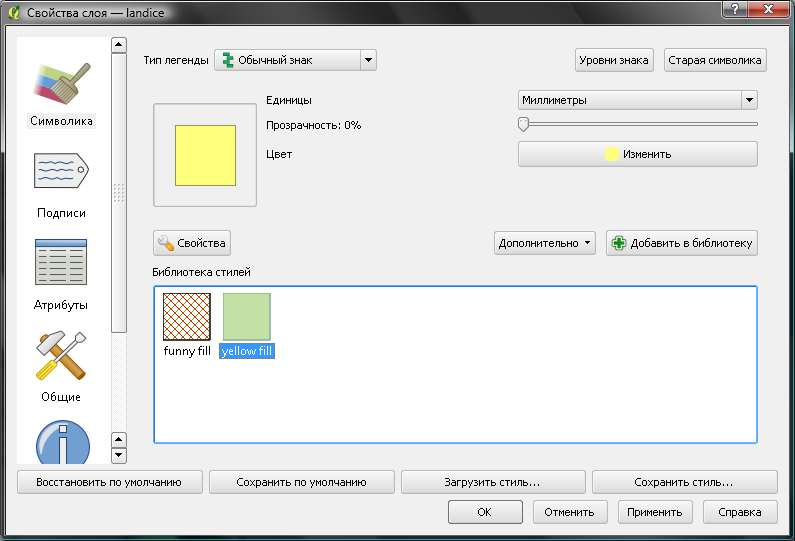
\includegraphics[clip=true, width=0.3\textwidth]{singlesymbol_ng_area}}
\caption{New Single Symbolizing options \nixcaption}
\end{figure}

\minisec{Categorized Renderer}

The Categorized Renderer is used to render all features from a layer, using a
single user-defined symbol, which color reflects the value of a selected
feature's attribute. The Symbology tab allows you to select:

\begin{itemize}[label=--]
\item The attribute (using the Column listbox)
\item The symbol (using the Symbol Properties dialog)
\item The colors (using the Color Ramp listbox)
\end{itemize}

For convenience, the list in the bottom part of the tab lists the values of
all currently selected attributes together, including the symbols that will
be rendered.

The example in figure \ref{fig:catsymNG} shows the category rendering dialog
used for the rivers layer of the \qg sample dataset.

\begin{figure}[ht]
   \centering
   \caption{New Categorized Symbolizing options \nixcaption}\label{fig:catsymNG}
   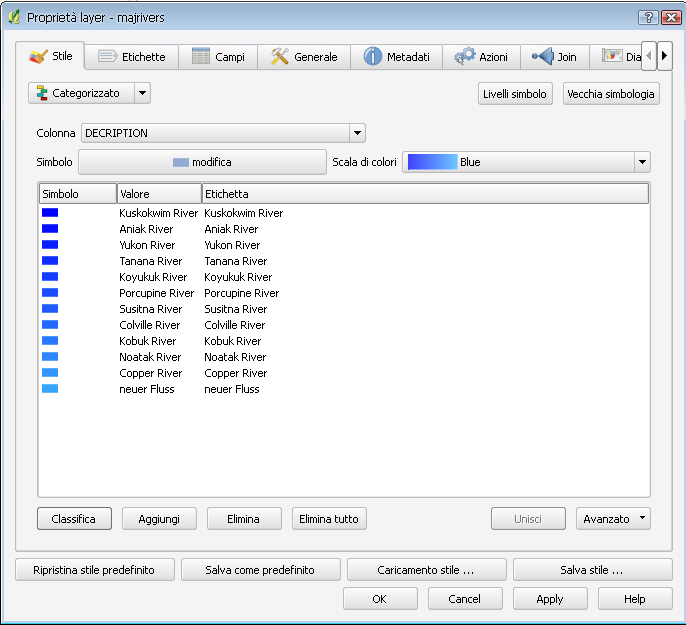
\includegraphics[clip=true, width=10cm]{categorysymbol_ng_line}
\end{figure}

\minisec{Graduated rendering}

The Graduated Renderer is used to render all the features from a layer, using
a single user-defined symbol, whose color reflects the classification of a selected
feature's attribute to a class.

Analogue to the categorized rendered, the symbology tab allows you to select:

\begin{itemize}[label=--]
\item The attribute (using the Column listbox)
\item The symbol (using the Symbol Properties button)
\item The colors (using the Color Ramp list)
\end{itemize}

Additionally, you can specify the number of classes and also the mode how to
classify features inside the classes (using the Mode list). The listbox in the
bottom part of the symbology tab lists the classes together with their ranges,
labels and symbols that will be rendered.

The example in figure \ref{fig:gradsymNG} shows the graduated rendering dialog
for the rivers layer of the \qg sample dataset.

\begin{figure}[ht]
   \centering
   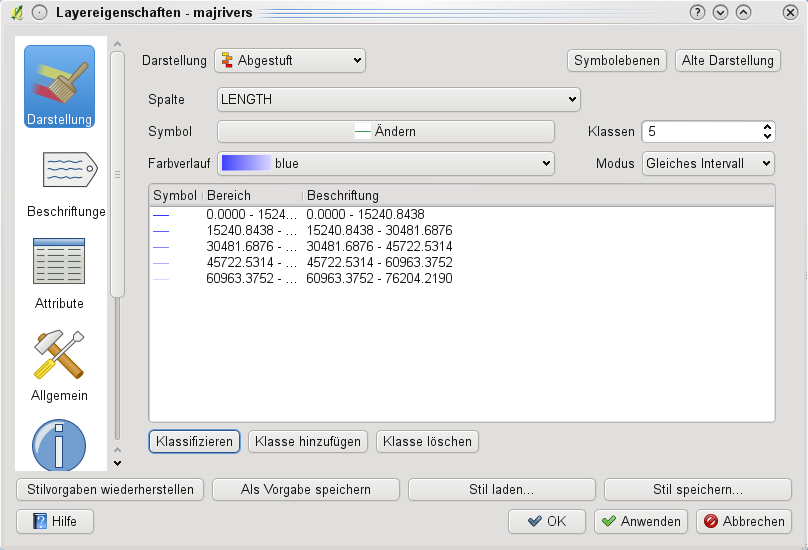
\includegraphics[clip=true, width=10cm]{graduatesymbol_ng_line}
   \caption{New Graduated Symbolizing options \nixcaption}\label{fig:gradsymNG}
\end{figure}

\minisec{Rule-based rendering}

The rule-based renderer is used to render all the features from a layer, using
rule based symbols, whose color reflects the classification of a selected
feature's attribute to a class.

%%FIXME
Add more text here

The example in figure \ref{fig:rulesymNG} shows the rule-based rendering dialog
for the rivers layer of the \qg sample dataset.

\begin{figure}[ht]
   \centering
   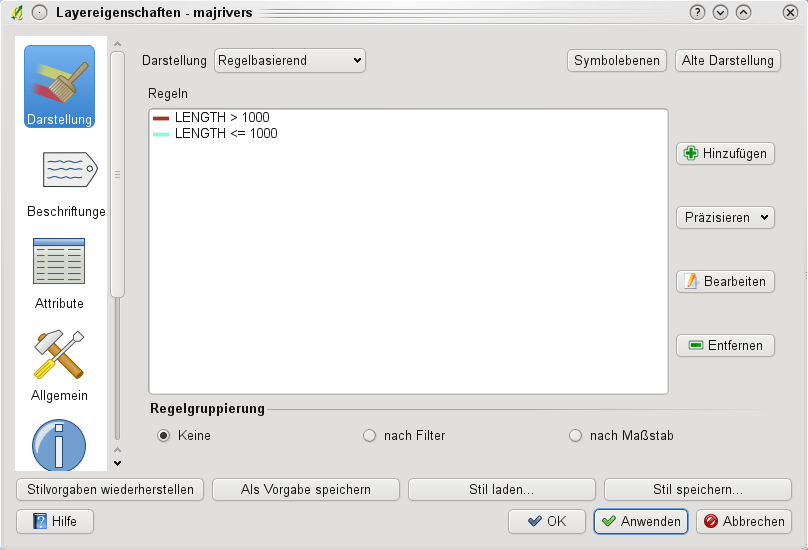
\includegraphics[clip=true, width=10cm]{rulesymbol_ng_line}
   \caption{New Rule-rBased Symbolizing options \nixcaption}\label{fig:rulesymNG}
\end{figure}

\minisec{Symbol Properties}

The symbol properties dialog allows the user to specify different properties of
the symbol to be rendered. In the top left part of the dialog, you find a preview
of the current symbol as it will be displayed in the map canvas. Below the preview
is the list of symbol layers. To start the symbol properties dialog, click the
\dropmenuopttwo{mActionOptions}{Properties} button in the \tab{Symbology} tab of the
\dialog{Layer Properties} dialog.

The control panels allow adding or removing layers, changing the position of layers,
or locking layers for color changes. In the right part of the dialog, there are
shown the settings applicable to the single symbol layer selected in the symbol
layer list. The most important is the 'Symbol Layer Type' combo box, which allows
you to choose the layer type. The available options depend on the layer type
(Point, Line, Polygon).

\begin{description}
\item Symbol layer type options for point layers
\begin{itemize}[label=--]
\item \textbf{SimpleMarker}: Border color, Fill color, Size, Angle, Offset X,Y
\item \textbf{SvgMarker}: Size, Angle, Offset X,Y, SVG Image
\end{itemize}
\item Symbol layer type options for line layers
\begin{itemize}[label=--]
\item \textbf{LineDecoration}: Color
\item \textbf{MarkerLine}: Marker, Marker Interval, Rotate marker, Line offset
\item \textbf{SimpleLine}: Color, Pen width, pen style, Offset, Join style and Cap style
\end{itemize}
\item Symbol layer type options for polygon layers
\begin{itemize}[label=--]
\item \textbf{SimpleFill}: Color, Fill style, Border color, Border style, Border width
\end{itemize}
\end{description}


\begin{figure}[ht]
\centering
   \subfloat[Line composed from three simple lines] {\label{subfig:symprops1}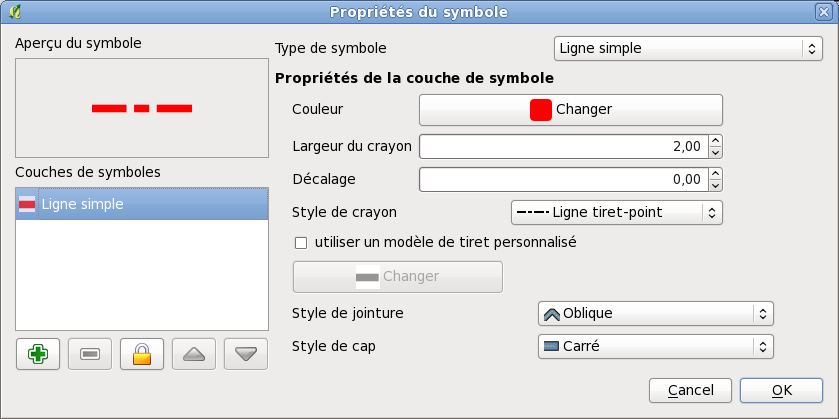
\includegraphics[clip=true, width=0.3\textwidth]{symbolproperties1}}
   \hspace{1cm}
   \subfloat[Symbol properties for point layer] {\label{subfig:symprops2}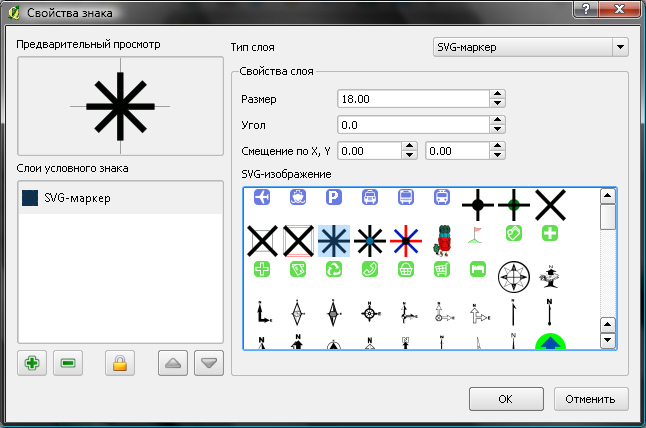
\includegraphics[clip=true, width=0.3\textwidth]{symbolproperties2}}
   \hspace{1cm}
   \subfloat[Filling pattern for a polygon] {\label{subfig:symprops3}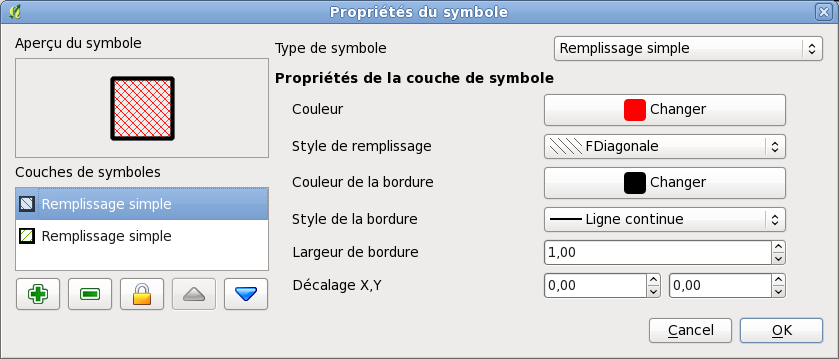
\includegraphics[clip=true, width=0.3\textwidth]{symbolproperties3}}
\caption{Defining symbol properties \nixcaption}
\end{figure}

\subsection{Style Manager to manage symbols and color ramps}\label{subsec:stylemanager}

The Style Manger is a small helper application, that lists symbols and color
ramps available in a style. It also allows you to add and/or remove items. To
launch the Style Manager, click on \mainmenuopt{Settings} > \dropmenuopt{Style
Manager} in the main menu.

\begin{figure}[ht]
   \centering
   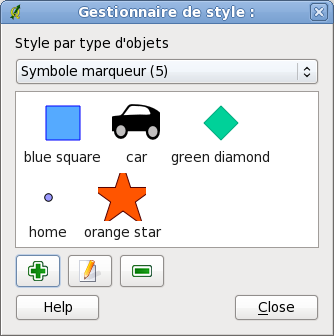
\includegraphics[clip=true, width=7cm]{stylemanager}
   \caption{Style Manager to manage symbols and color ramps \nixcaption}\label{fig:stylemanager}
\end{figure}

\subsection{Labels Tab}\label{labeltab}

The \tab{Labels} tab allows you to enable labeling features and control a number of
options related to fonts, placement, style, alignment and buffering.

We will illustrate this by labelling the lakes shapefile of the
\filename{\qg\_example\_dataset}:

\begin{enumerate}
\item Load the Shapefile \filename{alaska.shp} and GML file \filename{lakes.gml} in \qg.
\item Zoom in a bit to your favorite area with some lake.
\item Make the \filename{lakes} layer active.
\item Open the \dialog{Layer Properties} dialog.
\item Click on the \tab{Labels} tab.
\item Check the \checkbox{Display labels} checkbox to enable labeling.
\item Choose the field to label with.
  We'll use \selectstring{Field containing label}{NAMES}.
\item Enter a default for lakes that have no name. The default label will be
  used each time \qg encounters a lake with no value in the \guilabel{NAMES}
field.
\item If have labels extending over several lines, check \checkbox{Multiline
labels?}. \qg will check for a true line return in your label field and
insert the line breaks accordingly. A true line return is a \textbf{single}
character \textbackslash n, (not two separate characters, like a backlash
\textbackslash ~followed by the character n).
\item Click \button{Apply}.
\end{enumerate}

Now we have labels. How do they look? They are probably too big and poorly
placed in relation to the marker symbol for the lakes.

Select the \tab{Font} entry and use the \button{Font} and \button{Color}
buttons to set the font and color. You can also change the angle and the
placement of the text-label.

To change the position of the text relative to the feature:

\begin{enumerate}
\item Click on the \tab{Font} entry.
\item Change the placement by selecting one of the radio buttons
in the \classname{Placement} group. To fix our labels, choose the
\radiobuttonon{Right} radio button.
\item the \classname{Font size units} allows you to select between
\radiobuttonon{Points} or \radiobuttonon{Map units}.
\item Click \button{Apply} to see your changes without closing the dialog.
\end{enumerate}

Things are looking better, but the labels are still too close to the marker. To
fix this we can use the options on the \tab{Position} entry. Here we can add
offsets for the X and Y directions. Adding an X offset of 5 will move our
labels off the marker and make them more readable. Of course if your marker
symbol or font is larger, more of an offset will be required.

The last adjustment we'll make is to \tab{buffer} the labels. This just means
putting a backdrop around them to make them stand out better. To buffer the
lakes labels:

\begin{enumerate}
\item Click the \tab{Buffer} tab.
\item Click the \checkbox{Buffer Labels?} checkbox to enable buffering.
\item Choose a size for the buffer using the spin box.
\item Choose a color by clicking on \button{Color} and choosing your
  favorite from the color selector. You can also set some transparency for the
  buffer if you prefer.
\item Click \button{Apply} to see if you like the changes.
\end{enumerate}

If you aren't happy with the results, tweak the settings and then test again
by clicking \button{Apply}.

A buffer of 1 points seems to give a good result.
Notice you can also specify the buffer size in map units if that works out
better for you.

The remaining entries inside the \tab{Label} tab allow you control the appearance of the
labels using attributes stored in the layer. The entries beginning with \tab{Data defined} allow you to
set all the parameters for the labels using fields in the layer.

Not that the \tab{Label} tab provides a \classname{preview-box} where your
selected label is shown.

\subsection{New Labeling}\index{New labeling}\label{newlabel}

The new \toolbtntwo{labeling}{Labeling} core application provides smart labeling
for vector point, line and polygon layers and only requires a few parameters.
This new application will replace the current QGIS labeling, described in section
\ref{labeltab} and also supports on-the-fly transformated layers.

\minisec{Using new labeling}

\begin{enumerate}
  \item Start QGIS and load a vector point, line or polygon layer.
  \item Activate the layer in the legend and click on the
  \toolbtntwo{labeling}{Labeling} icon in the QGIS toolbar menu.
\end{enumerate}

\minisec{Labeling point layers}

First step is to activate the \checkbox{Label this layer} checkbox and select an attribute
column to use for labeling. After that you can define the label placement and text style,
labeling priority, scale-based visibility, if every part of multipart feature is to be
labeled and if features act as obstacles for labels or not (see
Figure \ref{fig:pointlabel}).

\begin{figure}[ht]
\centering
   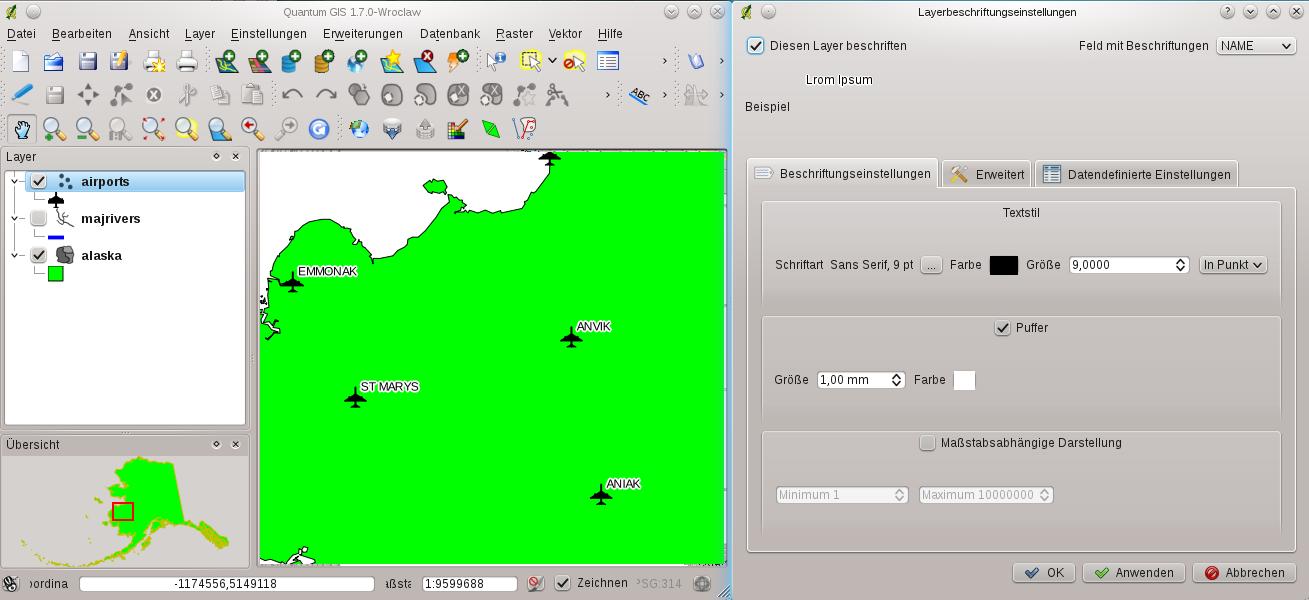
\includegraphics[clip=true, width=10cm]{label_points}
   \caption{Smart labeling of vector point layers \nixcaption}\label{fig:pointlabel}
\end{figure}

\minisec{Labeling line layers}

First step is to activate the \checkbox{Label this layer} checkbox and select an attribute
column to use for labeling. After that you can define the label placement, orientation,
distance to feature, text style, labeling priority, scale-based visibility, if every part
of a multipart line is to be labeled, if lines shall be merged to avoid duplicate labels
and if features act as obstacles for labels or not (see Figure \ref{fig:linelabel}).

\begin{figure}[ht]
\centering
   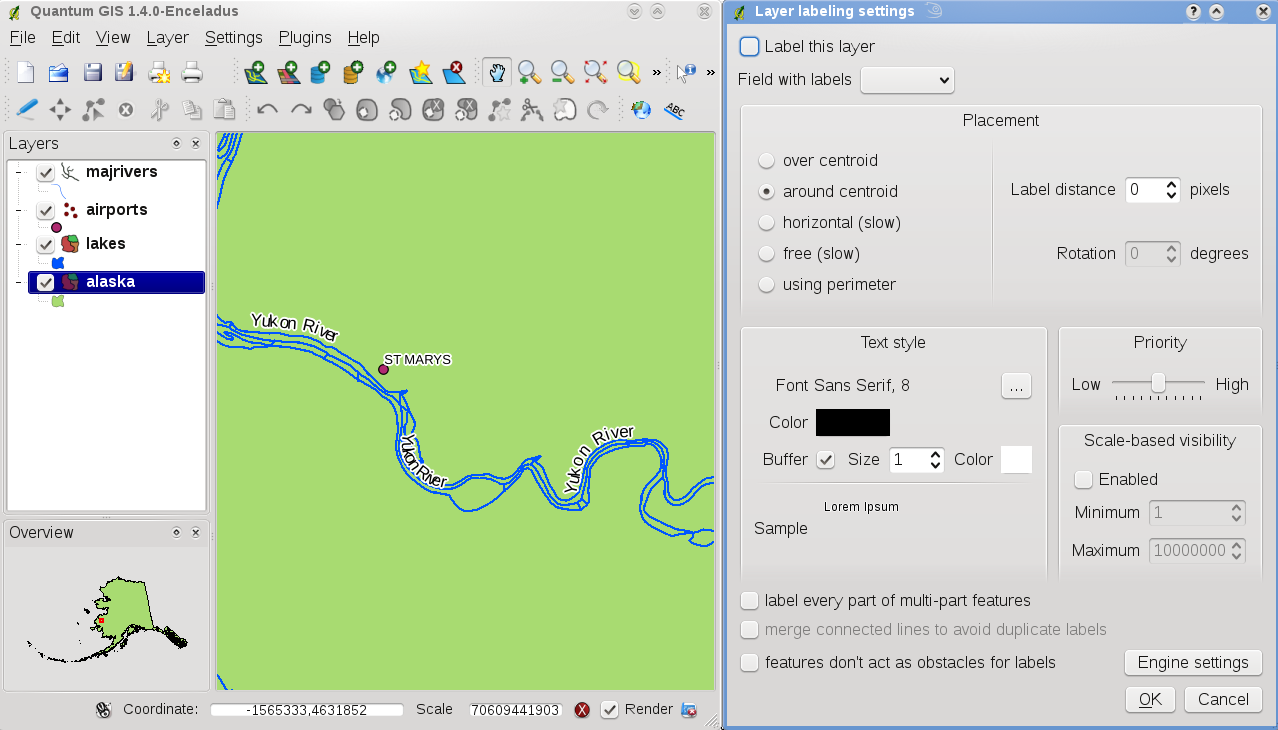
\includegraphics[clip=true, width=10cm]{label_line}
   \caption{Smart labeling of vector line layers \nixcaption}\label{fig:linelabel}
\end{figure}

\minisec{Labeling polygon layers}

First step is to activate the \checkbox{Label this layer} checkbox and select an attribute
column to use for labeling. After that you can define the label placement, distance and text
style, labeling priority, scale-based visibility, if every part of multipart feature is to be
labeled and if features act as obstacles for labels or not (see Figure \ref{fig:arealabel}).

\begin{figure}[ht]
\centering
   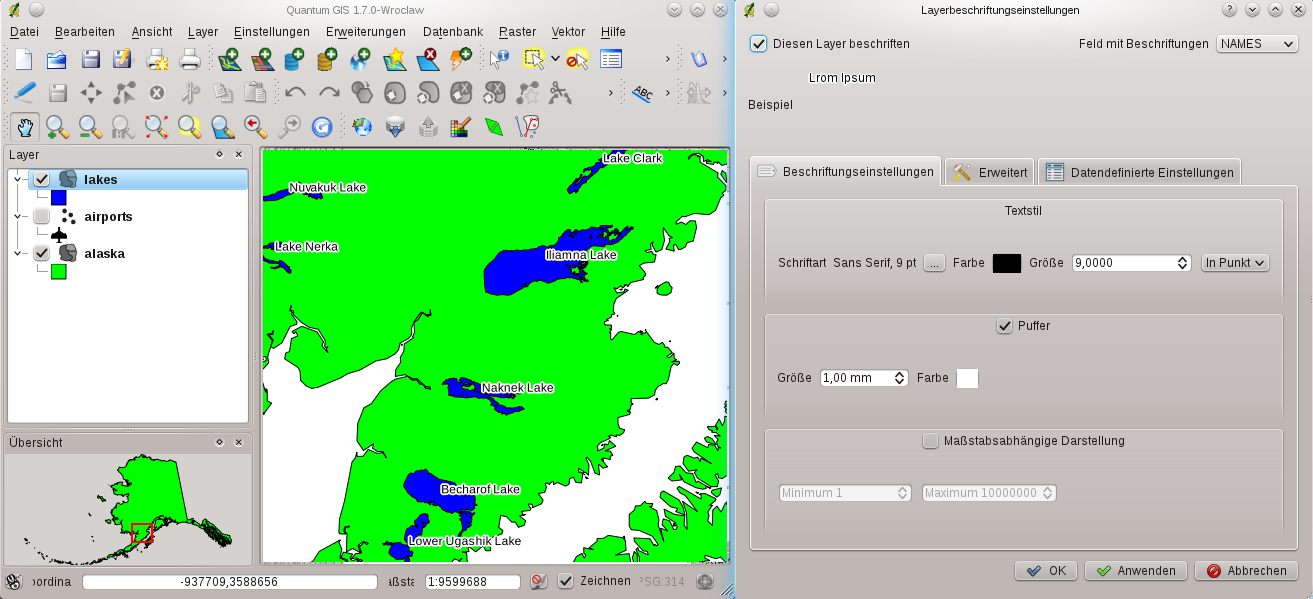
\includegraphics[clip=true, width=10cm]{label_area}
   \caption{Smart labeling of vector polygon layers \nixcaption}\label{fig:arealabel}
\end{figure}

\minisec{Change engine settings}

Additionally you can click the \button{Engine settings} button and select the search method,
used to find the best label placement. Available is Chain, Popmusic Tabu, Popmusic Chain,
Popmusic Tabu Chain and FALP.

\begin{figure}[ht]
\centering
   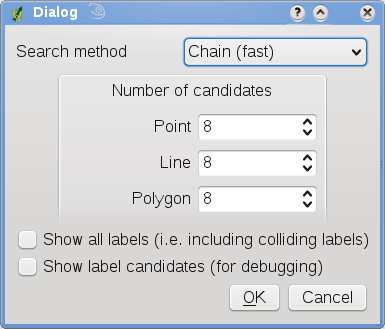
\includegraphics[clip=true, width=5cm]{label_engine}
   \caption{Dialog to change label engine settings \nixcaption}\label{fig:labelengine}
\end{figure}

Furthermore the number of candidates can be defined for point, line and polygon features,
and you can define whether to show all labels (including colliding labels) and label
candidates for debugging.

\subsection{Attributes Tab}\index{Attributes}\label{label_attributes}

Within the \tab{Attributes} tab the attributes of the selected dataset can be
manipulated. The buttons \toolbtntwo{mActionNewAttribute}{New Column} and
\toolbtntwo{mActionDeleteAttribute}{Delete Column} can be
used, when the dataset is \toolbtntwo{mActionToggleEditing}{editing mode}.
At the moment only columns from PostGIS layers can be removed and added. The
OGR library supports to add new columns, but not to remove them, if you have
a GDAL version >= 1.6 installed.

\minisec{edit widget}

\begin{figure}[ht]
   \centering
   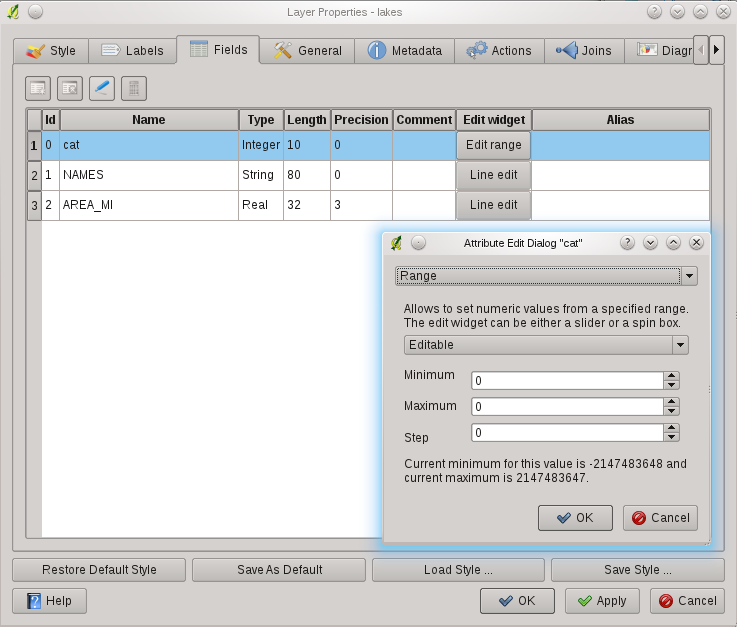
\includegraphics[clip=true, width=12cm]{editwidgetsdialog}
   \caption{Dialog to select an edit widget for an attribute column
\nixcaption}\label{fig:editwidget}
\end{figure}

Within the \tab{Attributes} tab you also find an \texttt{edit widget} column.
This column can be used to define values or a range of values that are
allowed
to be added to the specific attribute table column. If you click on the
\button{edit widget} button, a dialog opens, where you can define different
widgets. These widgets are:

\begin{itemize}[label=--]
\item Line edit: an edit field which allows to enter simple text (or restrict
to
numbers for numeric attributes).
\item Classification: Displays a combo box with the values used for
classification, if you have chosen 'unique value' as legend type in the
symbology tab of the properties dialog.
\item Range: Allows to set numeric values from a specific range. The edit
widget can be either a slider or a spin box.
\item Unique value: The user can select one of the values already used in the
attribute table. If editable is activated, a line edit is shown with
autocompletion support, otherwise a combo box is used.
\item File name: Simplifies the selection by adding a file chooser dialog.
\item Value map: a combo box with predefined items. The value is stored in
the attribute, the description is shown in the comboo box. You can define
values manually or load them from a layer or a csv file.
\item Enumeration: Opens a combo box with values that can be used within the
columns type. This is currently only supported by the postgres provider.
\item Immutable: The immutable attribute column is read-only. The user is not
able to modify the content.
\end{itemize}

\subsection{General Tab}\label{vectorgeneraltab}

The \tab{General} tab is essentially like that of the raster dialog. It
allows you to change the display name, set scale dependent rendering options,
create a spatial index of the vector file (only for OGR supported formats and
PostGIS) and view or change the projection of the specific vetor layer.

The \button{Query Builder} button allows you to create a subset of the
features in the layer - but this button currently only is available when you
open the attribute table and select the \button{...} button next to Advanced
search.

\subsection{Metadata Tab}\index{Metadata}

The \tab{Metadata} tab contains general information about the layer,
including specifics about the type and location, number of features, feature
type, and the editing capabilities. The \guiheading{Extents} section,
providing
layer extent information, and the \guiheading{Layer Spatial Reference System}
section, providing information about the CRS of the layer. This is a quick
way to get information about the layer, but is not yet editable.

\subsection{Actions Tab}\index{Actions}\label{label_actions}

\qg provides the ability to perform an action based on the attributes of a
feature. This can be used to perform any number of actions, for example,
running a program with arguments built from the attributes of a feature or
passing parameters to a web reporting tool.

Actions are useful when you frequently want to run an external application or
view a web page based on one or more values in your vector layer. An example
is performing a search based on an attribute value. This concept is used in
the following discussion.

\minisec{Defining Actions}\index{actions!defining}

Attribute actions are defined from the vector \dialog{Layer Properties} dialog. To
define an action, open the vector \dialog{Layer Properties} dialog and click on the
\tab{Actions} tab. Provide a descriptive name for the action. The action
itself must contain the name of the application that will be executed when the
action is invoked. You can add one or more attribute field values as arguments
to the application. When the action is invoked any set of characters that
start with a \% followed by the name of a field will be replaced by the value of
that field. The special characters \%\% \index{\%\%}will be replaced by the value
of the field that was selected from the identify results or attribute table (see
Using Actions below).  Double quote marks can be used to group text into a
single argument to the program, script or command. Double quotes will be
ignored if preceded by a backslash.

If you have field names that are substrings of other field names (e.g., \usertext{col1}
and \usertext{col10}) you should
indicate so, by surrounding the field name (and the \% character) with square
brackets (e.g., \usertext{[\%col10]}). This will prevent the \usertext{\%col10} field
name being mistaken for the \usertext{\%col1} field name with a \usertext{0}
on the end. The brackets will be removed by \qg when it substitutes in the
value of the field. If you want the substituted field to be surrounded by square
brackets, use a second set like this: \usertext{[[\%col10]]}.

The \dialog{Identify Results} dialog box includes a {\em (Derived)} item that
contains information relevant to the layer type. The
values in this item can be accessed in a similar way to the other fields
by using preceeding the derived field name by \usertext{(Derived).}. For
example, a point layer has an \usertext{X} and \usertext{Y} field and the
value of these can be used in the action with \usertext{\%(Derived).X} and
\usertext{\%(Derived).Y}. The derived attributes are only available from the
\dialog{Identify Results} dialog box, not the \dialog{Attribute Table} dialog box.

Two example actions are shown below:\index{actions!examples}

\begin{itemize}[label=--]
  \item \usertext{konqueror http://www.google.com/search?q=\%nam}
  \item \usertext{konqueror http://www.google.com/search?q=\%\%}
\end{itemize}

In the first example, the web browser konqueror is invoked and passed a URL to
open. The URL performs a Google search on the value of the \usertext{nam} field
from our vector layer. Note that the application or script called by the
action must be in the path or you must provided the full path. To be sure, we could
rewrite the first example as: \usertext{/opt/kde3/bin/konqueror
http://www.google.com/search?q=\%nam}. This will ensure that the konqueror
application will be executed when the action is invoked.

The second example uses the \%\% notation which does not rely on a particular
field for its value. When the action is invoked, the \%\% will be replaced by
the value of the selected field in the identify results or attribute table.

\minisec{Using Actions}\index{actions!using}\label{label_usingactions}

Actions can be invoked from either the \dialog{Identify Results} dialog or an
\dialog{Attribute Table} dialog. (Recall that these dialogs can be opened by
clicking \toolbtntwo{mActionIdentify}{Identify Features} or
\toolbtntwo{mActionOpenTable}{Open Attribute Table}.) To invoke an action,
right click on the record and choose the action from the popup menu. Actions
are listed in the popup menu by the name you assigned when defining the
actions. Click on the action you wish to invoke.

If you are invoking an action that uses the \%\% notation, right-click on the
field value in the \dialog{Identify Results} dialog or the
\dialog{Attribute Table} dialog that you wish to pass to the application or script.

Here is another example that pulls data out of a vector layer and inserts them
into a file using bash and the \usertext{echo} command (so it will only work
\nix or perhaps \osx). The layer in question has fields for a species name
\usertext{taxon\_name}, latitude \usertext{lat} and longitude
\usertext{long}. I would like to be able to
make a spatial selection of a localities and export these field values to a
text file for the selected record (shown in yellow in the \qg map area). Here is
the action to achieve this:

\begin{verbatim}
  bash -c "echo \"%taxon_name %lat %long\" >> /tmp/species_localities.txt"
\end{verbatim}

After selecting a few localities and running the action on each one, opening
the output file will show something like this:

\begin{verbatim}
  Acacia mearnsii -34.0800000000 150.0800000000
  Acacia mearnsii -34.9000000000 150.1200000000
  Acacia mearnsii -35.2200000000 149.9300000000
  Acacia mearnsii -32.2700000000 150.4100000000
\end{verbatim}

As an exercise we create an action that does a Google search on the
\filename{lakes} layer. First we need to determine the URL needed to perform a search on a
keyword. This is easily done by just going to Google and doing a simple
search, then grabbing the URL from the address bar in your browser. From this
little effort we see that the format is: \url{http://google.com/search?q=qgis},
where \usertext{\qg} is the search term. Armed with this information, we can
proceed:

\begin{enumerate}
\item Make sure the \filename{lakes} layer is loaded.
\item Open the \dialog{Layer Properties} dialog by double-clicking on the layer in the
  legend or right-click and choose \dropmenuopt{Properties} from the popup menu.
\item Click on the \tab{Actions} tab.
\item Enter a name for the action, for example \usertext{Google Search}.
\item For the action, we need to provide the name of the external program to
  run. In this case, we can use Firefox. If the program is not in
  your path, you need to provide the full path.
\item Following the name of the external application, add the URL used for
  doing a Google search, up to but not included the search term:
  \url{http://google.com/search?q=}
\item The text in the \guilabel{Action} field should now look like this:\\
  \usertext{firefox \url{http://google.com/search?q=}}
\item Click on the drop-down box containing the field names for the
  \usertext{lakes} layer. It's located just to the left of the
  \button{Insert Field} button.
\item From the drop-down box, select \selectstring{Field containing label}{NAMES} and click \button{Insert Field}.
\item Your action text now looks like this:\\ \usertext{firefox
  \url{http://google.com/search?q=\%NAMES}}
\item Fo finalize the action click the \button{Insert action} button.
\end{enumerate}

This completes the action and it is ready to use. The final text of the action
should look like this:

\usertext{firefox \url{http://google.com/search?q=\%NAMES}}

We can now use the action. Close the \dialog{Layer Properties} dialog and zoom in to an area
of interest. Make sure the \filename{lakes} layer is active and identify a
lake. In the result box you'll now see that our action is visible:

\begin{figure}[ht]
   \centering
   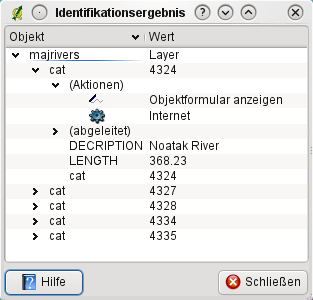
\includegraphics[clip=true, width=7cm]{action_identifyaction}
   \caption{Select feature and choose action \nixcaption}\label{fig:identify_action}
\end{figure}

When we click on the action, it brings up Firefox and navigates to the URL
\url{http://www.google.com/search?q=Tustumena}. It is also possible to add further
attribute fields to the action. Therefore you can add a ``+'' to the end of the action
text, select another field and click on \button{Insert Field}. In this example there
is just no other field available that would make sense to search for.

You can define multiple actions for a layer and each will show up in the
\dialog{Identify Results} dialog.
%% FIXME No longer valid??
%%You can also invoke actions from the attribute table
%%by selecting a row and right-clicking, then choosing the action from the popup
%%menu.

You can think of all kinds of uses for actions. For example, if you have a point layer
containing locations of images or photos along with a file name, you could
create an action to launch a viewer to display the image. You could also use
actions to launch web-based reports for an attribute field or combination of
fields, specifying them in the same way we did in our Google search example.

\subsection{Diagram Tab}\label{sec:diagram}
\index{vector layers!diagram}

The \tab{Diagram} tab allows you to add a grahic overlay to a vector layer.
To activate this feature, open the Plugin Manager and select the Diagram Overlay'
plugin. After this, there is a new tab in the vector \dialog{Layer
Properties} dialog where the settings for diagrams may be entered (see
figure~\ref{fig:diagramtab}).

\begin{figure}[ht]
   \centering
   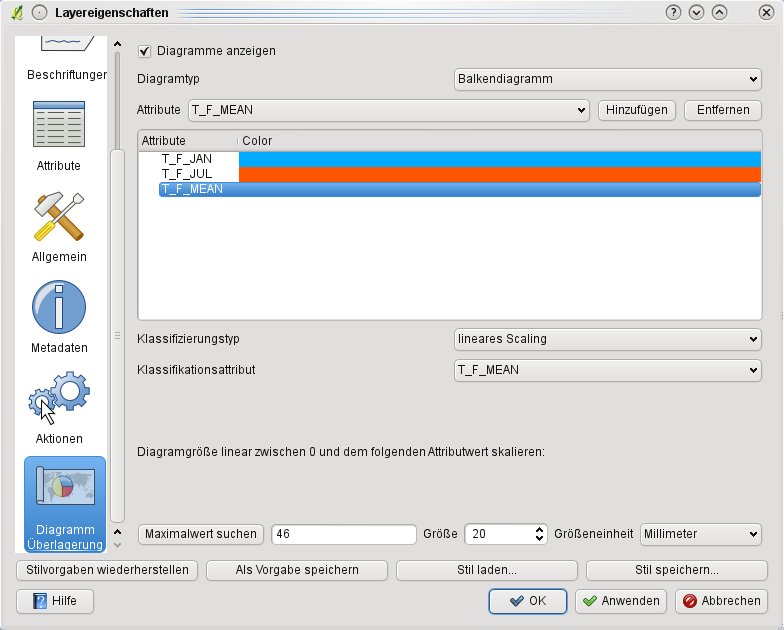
\includegraphics[clip=true, width=13cm]{diagram_tab}
   \caption{Vector properties dialog with diagram tab \nixcaption}\label{fig:diagramtab}
\end{figure}

The current implementation of diagrams provides support for piecharts, barcharts,
proportional SVG symbols, and for linear scaling of the diagram size according
to a classification attribute. We will demonstrate an example and overlay the
alaska boundary layer a barchart diagram showing some temperature data from
a climate vector layer. Both vector layers are part of the \qg sample dataset (see
Section~\ref{label_sampledata}.

\begin{enumerate}
\item First click on the \toolbtntwo{mActionAddOgrLayer}{Load Vector} icon,
browse to the \qg sample dataset folder and load the two vector shape layers
\filename{alaska.shp} and \filename{climate.shp}.
\item Double click the \filename{climate} layer in the map legend to open the
\dialog{Layer Properties} dialog.
\item Click on the \tab{Diagram Overlay} and select \button{Bar chart} as
Diagram type.
\item In the diagram we want to display the values of the three columns
\filename{T\_F\_JAN, T\_F\_JUL} and \filename{T\_F\_MEAN}. First select
\filename{T\_F\_JAN} as Attributes and click \button{Add attribute}, then
\filename{T\_F\_JUL} and finally \filename{T\_F\_MEAN}.
\item For linear scaling of the diagram size we define \filename{T\_F\_JUL}
as classification attribute.
\item Now click on \button{find maximum value}, choose a size value and unit
and click \button{Apply} to display the diagram in the \qg main window.
\item You can now adapt the chart size, or change the attribute colors double
clicking on the color values in the attribute field.
Figure~\ref{fig:climatediagram} gives an impression.
\item Finally click \button{Ok}.
\end{enumerate}

\begin{figure}[ht]
   \centering
   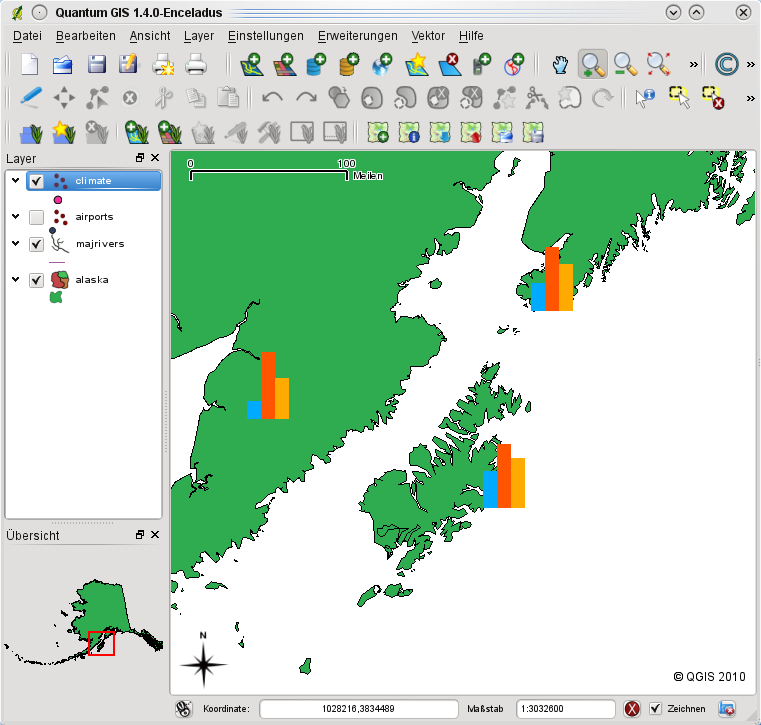
\includegraphics[clip=true, width=13cm]{climate_diagram}
   \caption{Diagram from temperature data overlayed on a map \nixcaption}\label{fig:climatediagram}
\end{figure}

\section{Редактирование}\index{editing}

\qg предоставляет разнообразные возможности для редактирования векторных
данных OGR, PostGIS и Spatialite. \textbf{Примечание} "--- процедура
редактирования данных GRASS имеет свои отличия "--- подробнее см.
Раздел~\ref{grass_digitising}.

\begin{Tip}\caption{\textsc{Параллельное редактирование}}
Данная версия \qg не различает между собой нескольких пользователей,
одновременно редактирующих одни и те же данные. Сохраняются изменения
того пользователя, который сохранил их последним.
\end{Tip}

\subsection{Настройка Порога Прилипания и Радиуса Поиска}\label{snapping_tolerance}

Перед началом редактирования узлов, необходимо установить величину порога
прилипания и радиуса поиска, что позволит оптимизировать редактирование
геометрии векторных слоев.

\minisec{Порог прилипания}

Порог прилипания "--- это расстояние, используемое \qg для \usertext{поиска}
ближайшего узла и/или сегмента, к которому надо присоединиться при создании
нового узла или передвижении уже существующего. Если превысить порог
прилипания \qg при нажатии кнопки мыши, то узел будет создан  в стороне,
вместо того, чтобы быть привязанным к уже существующему узлу и/или сегменту.
Величина порога прилипания оказывает влияние на функционирование всех
инструментов программы, связанных с величинами допуска.

\begin{enumerate}
\item Общая для всего проекта величина порога прилипания устанавливается в
\mainmenuopt{Установки} \arrow \dropmenuopttwo{mActionOptions}{Параметры}
(Для Mac: \mainmenuopt{\qg} \arrow Настройки, для Linux: \mainmenuopt{Редактирование}
\arrow \dropmenuopttwo{mActionOptions}{Параметры}).
На вкладке \tab{Оцифровка} можно установить режим прилипания по умолчанию: к
вершинам, к сегментам или к вершинам и сегментам. Также можно определить
значения по умолчанию для единиц измерения порога прилипания и радиуса поиска.
Эти величины  могут быть установлены как в единицах карты, так и в пикселах.
Преимущество использования пикселов в качестве единиц заключается в том, что
при зуммировании порог прилипания не будет изменяться.
В нашем небольшом проекте оцифровки (по рабочему набору данных Alaska), мы
установили в качестве единицы порога прилипания фут. Ваши результаты могут
отличаться, но величины близкие к 300 футов дают приемлемые
результаты при работе в масштабе 1:10~000.
\item Величина порога прилипания для отдельного слоя устанавливается в
\mainmenuopt{Установки} (или \mainmenuopt{File}) \arrow
\dropmenuopttwo{mActionOptions}{Свойства проекта\dots}. На вкладке \tab{Общие},
в секции \classname{Оцифровка} нажмите на \\
\button{Параметры прилипания\dots} для
включения и настройки режима и порога прилипания для каждого слоя (см.
Рисунок~\ref{fig:snappingoptions}).
\end{enumerate}
Обратите внимание, что величина порога прилипания для отдельного слоя
доминирует над общим порогом прилипания, установленным на вкладке «Оцифровка».
Таким образом, если надо отредактировать один слой и прилепить его вершины
к другому слою, необходимо активировать прилипание \usertext{прилипание к}
для слоя, затем снизить общий порог прилипания для проекта до меньшего
значения. Кроме того, прилипание невозможно для слоя, не активизированного
в диалоговом окне параметров прилипания, независимо от параметров
общего прилипания. Поэтому необходимо убедиться, что у слоя, к которому
необходимо использовать прилипание, стоит флажок.

\begin{figure}[ht]
   \centering
   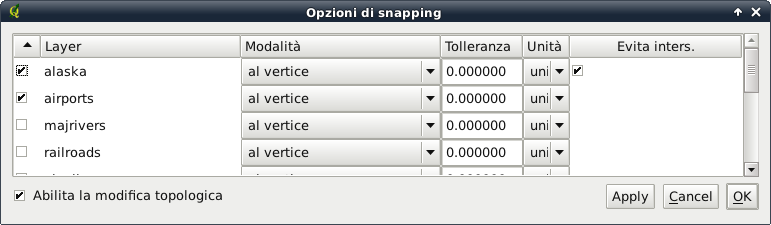
\includegraphics[clip=true, width=12cm]{editProjectSnapping}
   \caption{Установка параметров прилипания для отдельного слоя \nixcaption}\label{fig:snappingoptions}
\end{figure}

\minisec{Радиус поиска}

Радиус поиска "--- это расстояние \qg , используемое для \usertext{поиска}
ближайшей вершины, которую вы пытаетесь переместить, щелкая кнопкой мыши
по карте. За пределом радиуса поиска \qg не сможет найти и выделить
какую-либо вершину для последующего редактирования, о чем сообщит
всплывающее окно предупреждения. Порог прилипания и радиус поиска
устанавливаются в единицах карты или пикселях, для того, чтобы установить
приемлемые значения, лучше всего с ними поэкспериментировать. Если установлен
слишком большой порог, \qg может прилепиться к неверной вершине, особенно,
если работа идет с большим количеством близко расположенных вершин. Однако
слишком маленький порог не позволит обнаружить какой-либо объект.

Радиус поиска для редактирования вершин в единицах слоя устанавливается
на вкладке \tab{Оцифровка}, расположенной в \mainmenuopt{Установки} \arrow
\dropmenuopttwo{mActionOptions}{Параметры}. Там же устанавливается общий
для всего проекта порог прилипания.

\subsection{Зуммирование и прокрутка карты}

Перед редактированием слоя, следует увеличить район исследований на карте.
Это убережет от ожидания прорисовки всех вершин слоя.

Помимо использования кнопок \toolbtntwo{mActionPan}{Прокрутка карты} и
\toolbtntwo{mActionZoomIn}{Увеличить}/\toolbtntwo{mActionZoomOut}{Уменьшить}
на панели инструментов, навигация также может осуществляться с
помощью колесика мыши, клавиши «Пробел» и стрелок.

\minisec{Зуммирование и прокрутка карты с помощью колесика мыши}

Нажатие и удержание колесика мыши во время редактирования позволяет перемещать
карту в пределах основного окна,а прокручивание колесика мыши приводит к
масштабированию карты. Для увеличения необходимо расположить курсор мыши внутри
площади карты и крутить колесико вперед (от себя), для уменьшения "--- назад
(к себе). Положение курсора мыши является центром области зуммирования. Можно
настроить режим зуммирования колесиком мыши, используя вкладку
\tab{Инструменты} в меню \mainmenuopt{Установки} \arrow \dropmenuopt{Параметры}.

\minisec{Прокрутка карты с помощью стрелок}

Прокрутка карты во время редактирования возможна с помощью стрелок. Расположите
курсор мыши внутри площади карты и нажмите на правую стрелку для перемещения на
восток, на левую стрелку для перемещения на запад, стрелку вверх для перемещения на
север и стрелку вниз для перемещения на юг.

Также возможно использовать клавишу «Пробел» для временного замещения мыши при
прокрутке карты. Нажатие стрелок клавиатуры «Вверх» и «Вниз» приведет к
увеличению и уменьшению карты, не прерывая процесса оцифровки.

\subsubsection{Топологическое редактирование}

Кроме установки параметров прилипания для отдельного слоя, на вкладке \tab{Общее}
из меню
\mainmenuopt{Установки} \arrow \dropmenuopttwo{mActionOptions}{Свойства проекта\dots}
можно установить топологическое редактирование. В группе опций по Оцифровке
можно активировать \checkbox{Включить топологическое редактирование} и/или
также активировать \\
\checkbox{Предотвращать пересечение новых полигонов}.

\minisec{Включение топологического редактирования}

Опция \checkbox{Включить топологическое редактирование} предназначена для
редактирования и управления общими границами в мозаике полигонов. \qg
«определяет» общие границы в мозаике полигонов. При изменении положения
вершины одного полигона, \qg позаботится о том, чтобы положение вершины
соседнего полигона изменилось в соответствии.

\minisec{Предотвращение пересечения новых полигонов}

Следующая топологическая опция называется \checkbox{Предотвращение пересечения
новых полигонов} и позволяет избежать пересечений в мозаике полигонов, что
ускоряет редактрование смежных полигонов. Если один полигон уже существует,
с помощью этой функции можно оцифровать новый с пересечением первого, и
\qg обрежет второй полигон по общей границе. Основное преимущество заключается
в том, что пользователи не должны цифровать все вершины по границе смежных
полигонов.

\subsection{Редактирование существующего слоя}
\index{vector layers!digitizing}
\index{digitizing!an existing layer}
\label{sec:edit_existing_layer}

По умолчанию, \qg подгружает слои, делая их доступными только для чтения:
это защита от непреднамеренного редактирования слоя, что случается, например,
при выскальзывании мыши. Однако можно установить редактирование любого слоя,
при условии, если на это имеется соответствующее разрешение и основной
источник данных имеет возможность записи (т.\,е. эти файлы доступны не только
для чтения). Редактирование слоев наиболее универсально, если используются
источники данных, основанных на PostgreSQL/PostGIS.

Все возможности редактирования векторных слоев разделены между панелями
инструментов оцифровки и дополнительным функциям оцифровки, описанных в
Разделе~\ref{sec:advanced_edit}. Их можно активировать и деактивировать
в меню \mainmenuopt{Вид} \arrow \dropmenuopt{Панели инструментов}.
Используя основные инструменты для оцифровки, можно выполнять следующие
функции:

\begin{table}[ht]\index{vector layers!basic editing tools}
\centering
\begin{tabular}{|l|p{5.5cm}|l|p{5.5cm}|}
\hline \textbf{Иконка} & \textbf{Назначение} & \textbf{Иконка} & \textbf{Назначение} \\
\hline 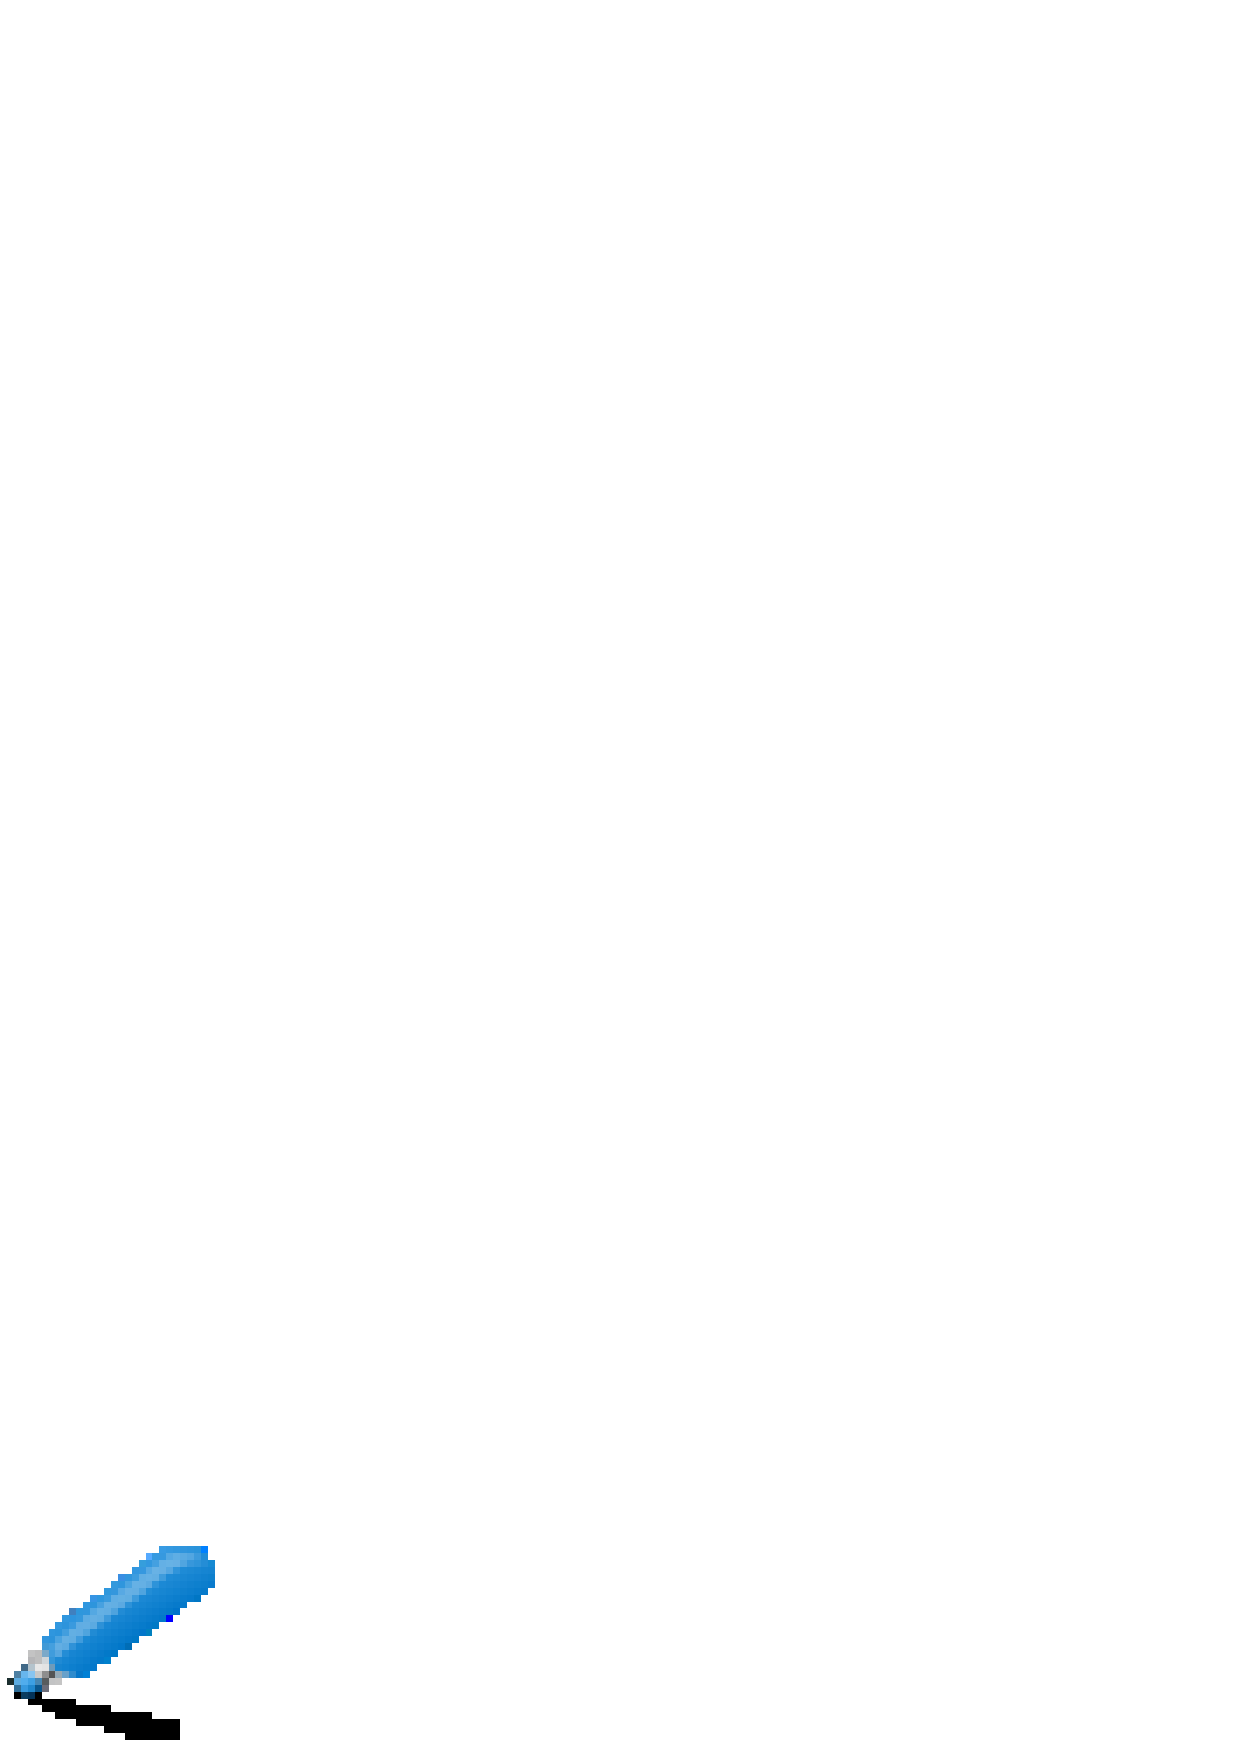
\includegraphics[width=0.7cm]{mActionToggleEditing}
   & Режим редактирования
   & 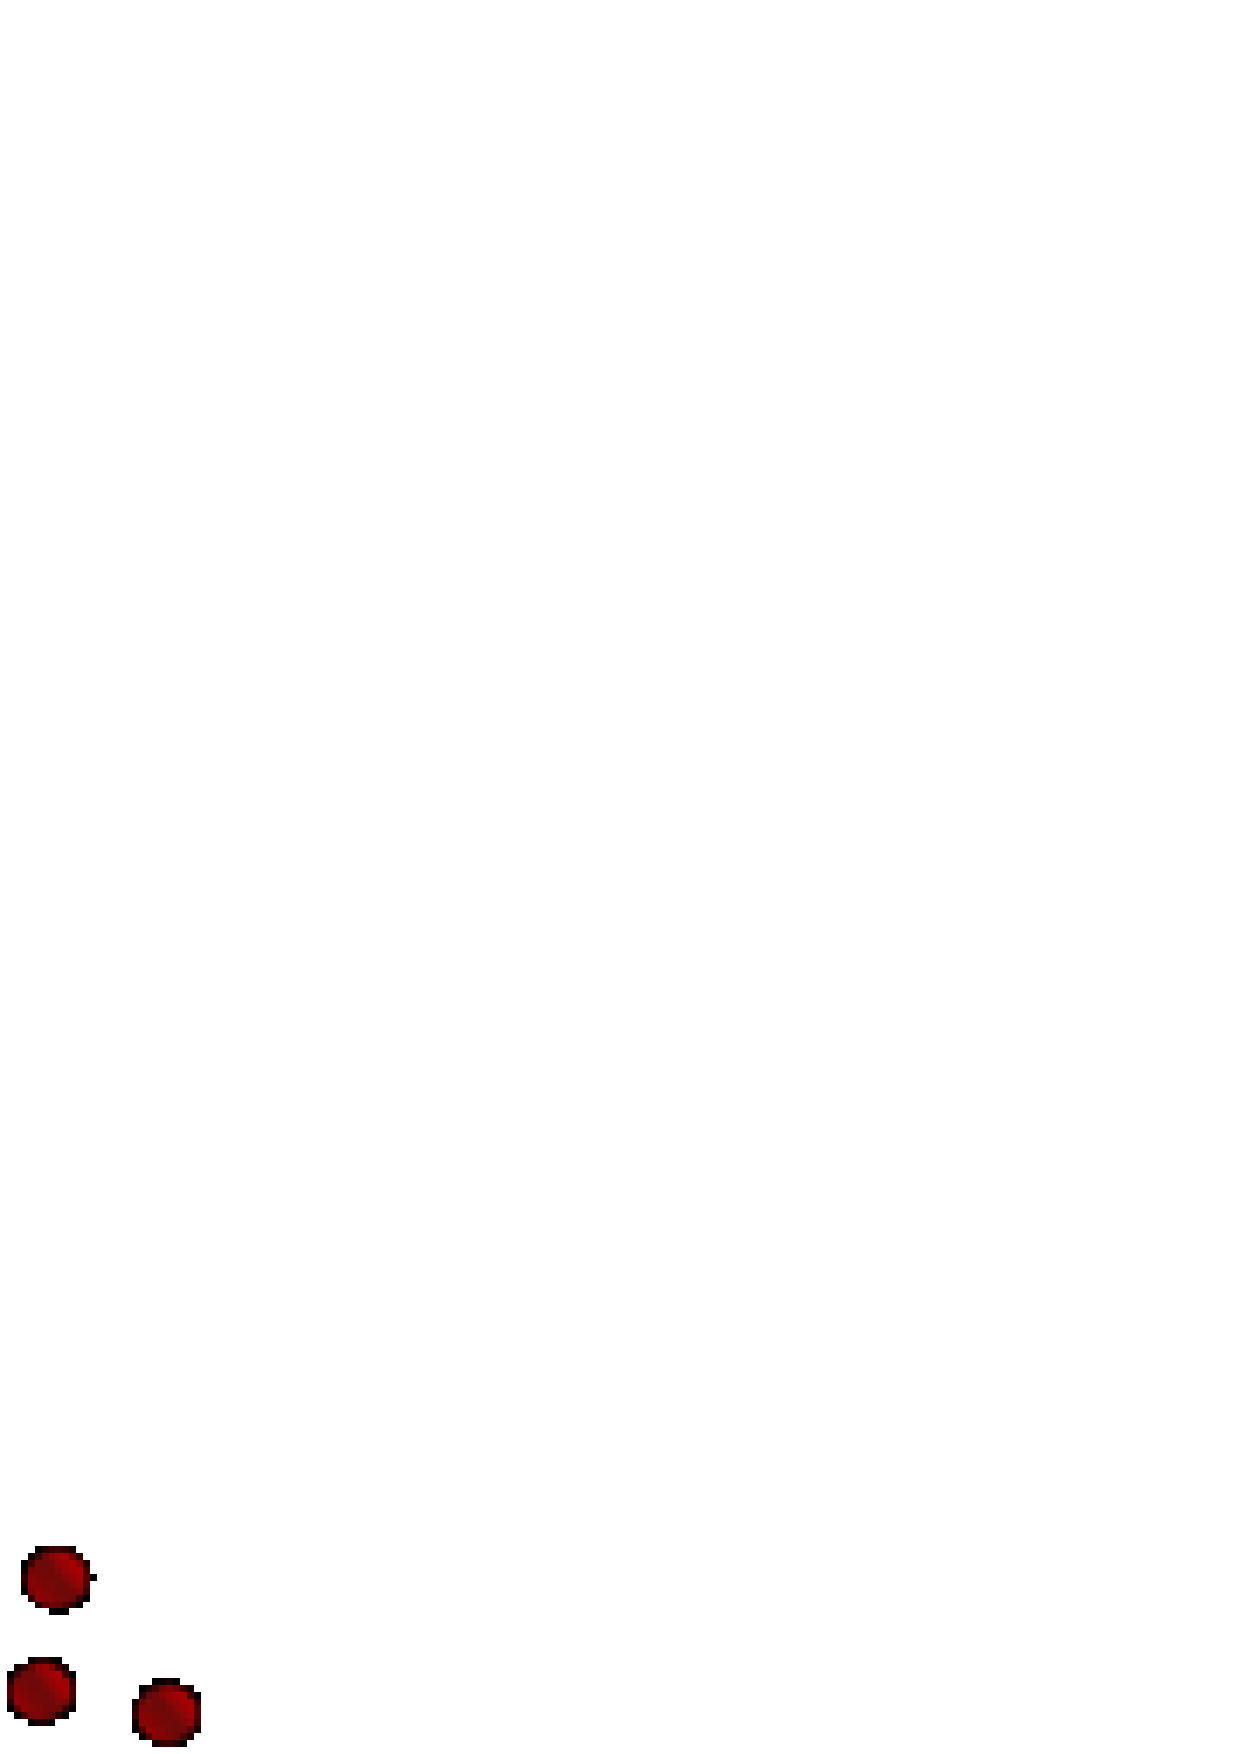
\includegraphics[width=0.7cm]{mActionCapturePoint}
   & Создать точку \\
\hline 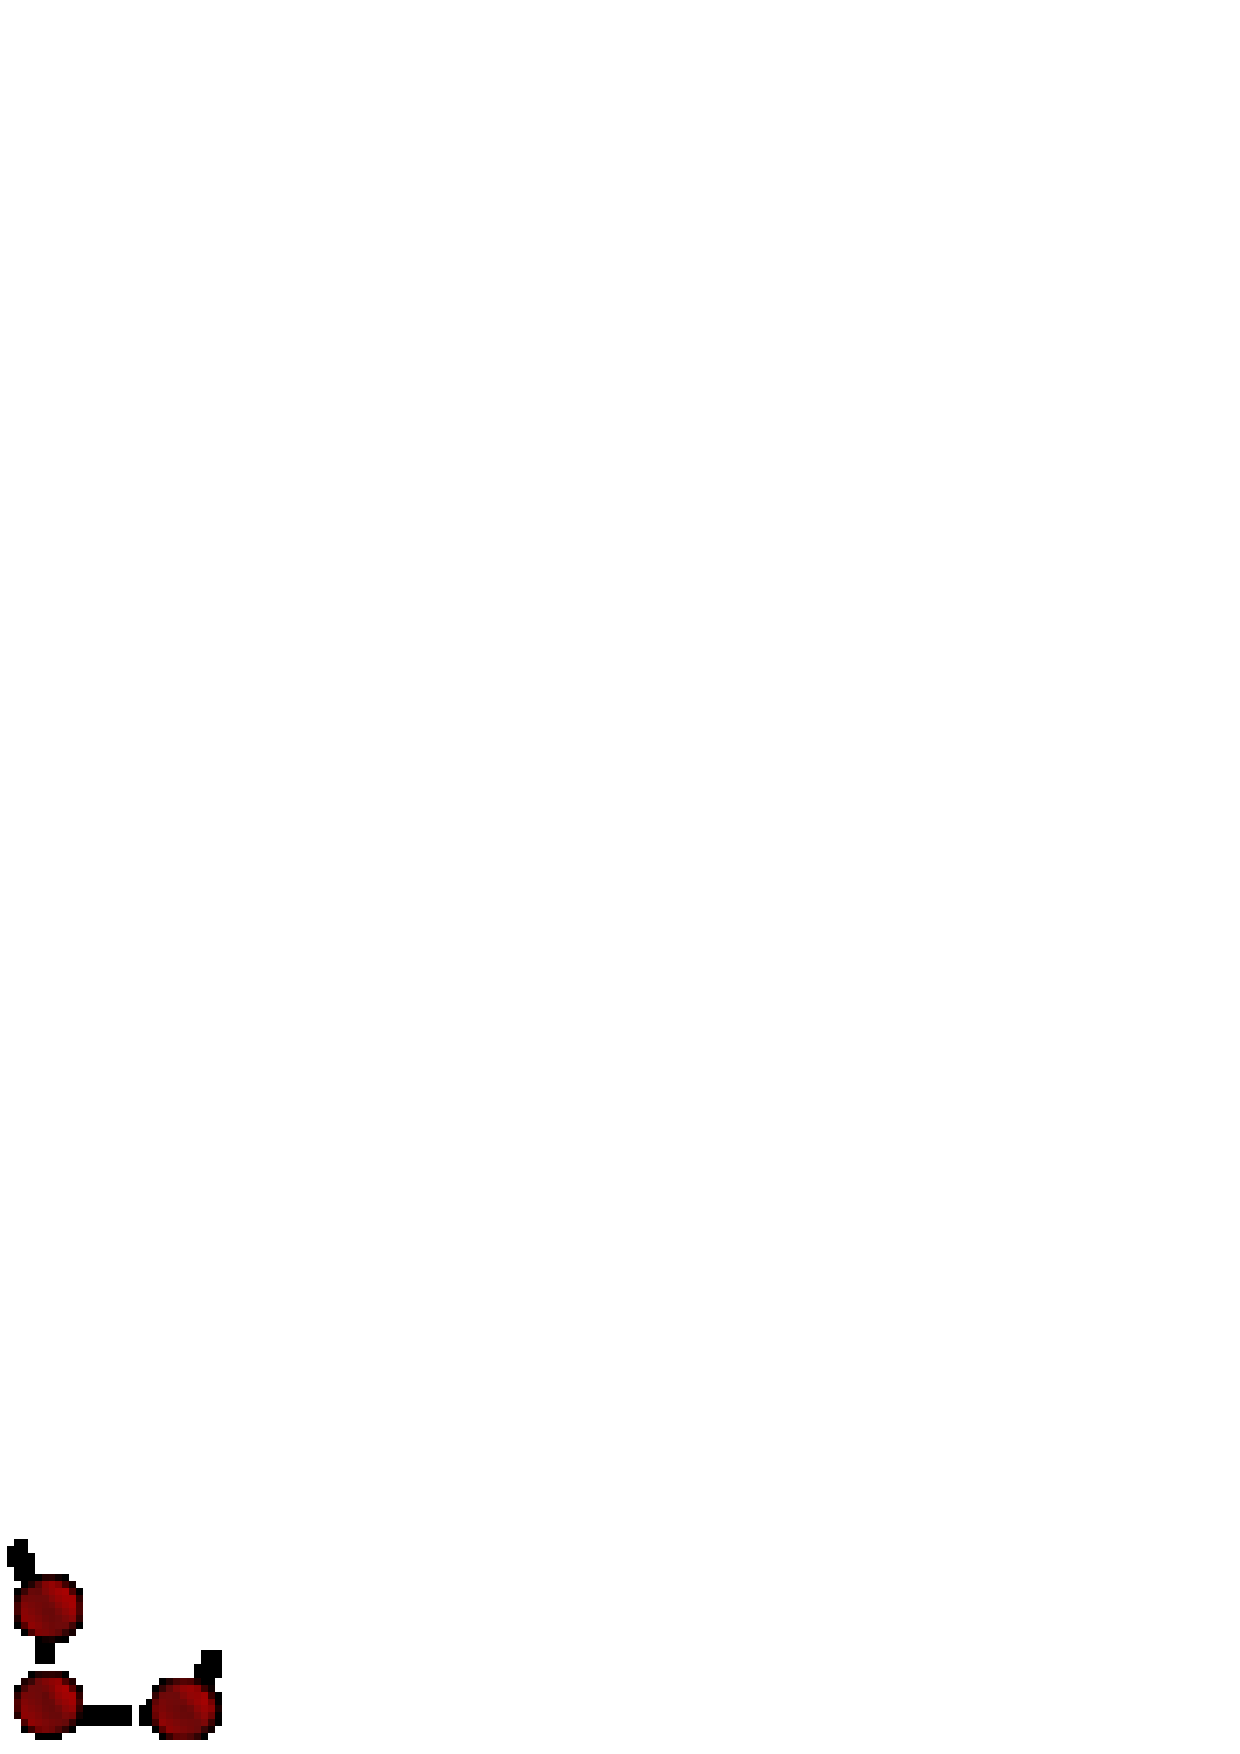
\includegraphics[width=0.7cm]{mActionCaptureLine}
   & Создать линию
   & 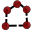
\includegraphics[width=0.7cm]{mActionCapturePolygon}
   & Создать полигон \\
\hline 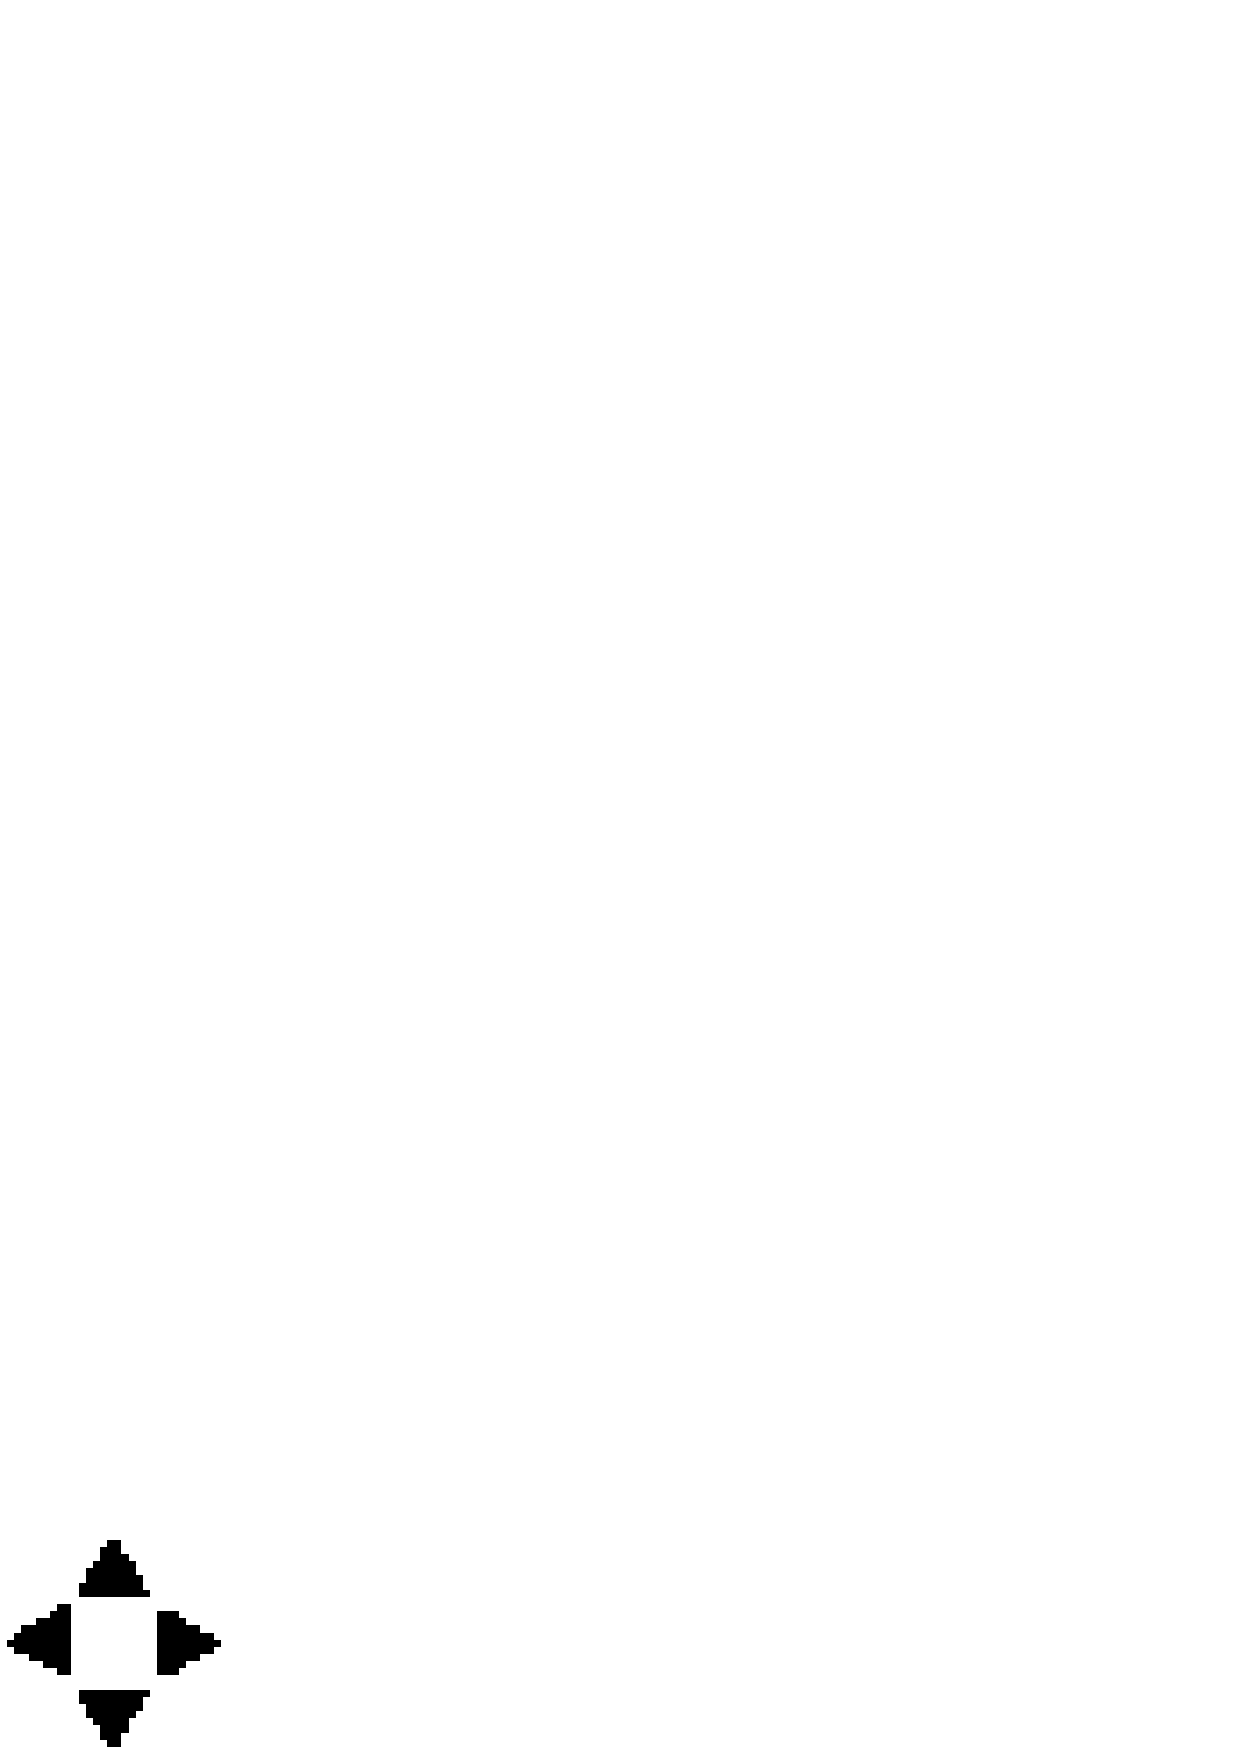
\includegraphics[width=0.7cm]{mActionMoveFeature}
   & Переместить объект
   & 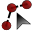
\includegraphics[width=0.7cm]{mActionNodeTool}
   & Редактирование узлов \\
\hline 
\includegraphics[width=0.7cm]{mActionDeleteSelected}
   & Удалить выделенное
   & 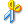
\includegraphics[width=0.7cm]{mActionEditCut}
   & Вырезать объекты \\
\hline 
\includegraphics[width=0.7cm]{mActionEditCopy}
   & Копировать объекты
   & 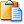
\includegraphics[width=0.7cm]{mActionEditPaste}
   & Вставить объекты \\
\hline 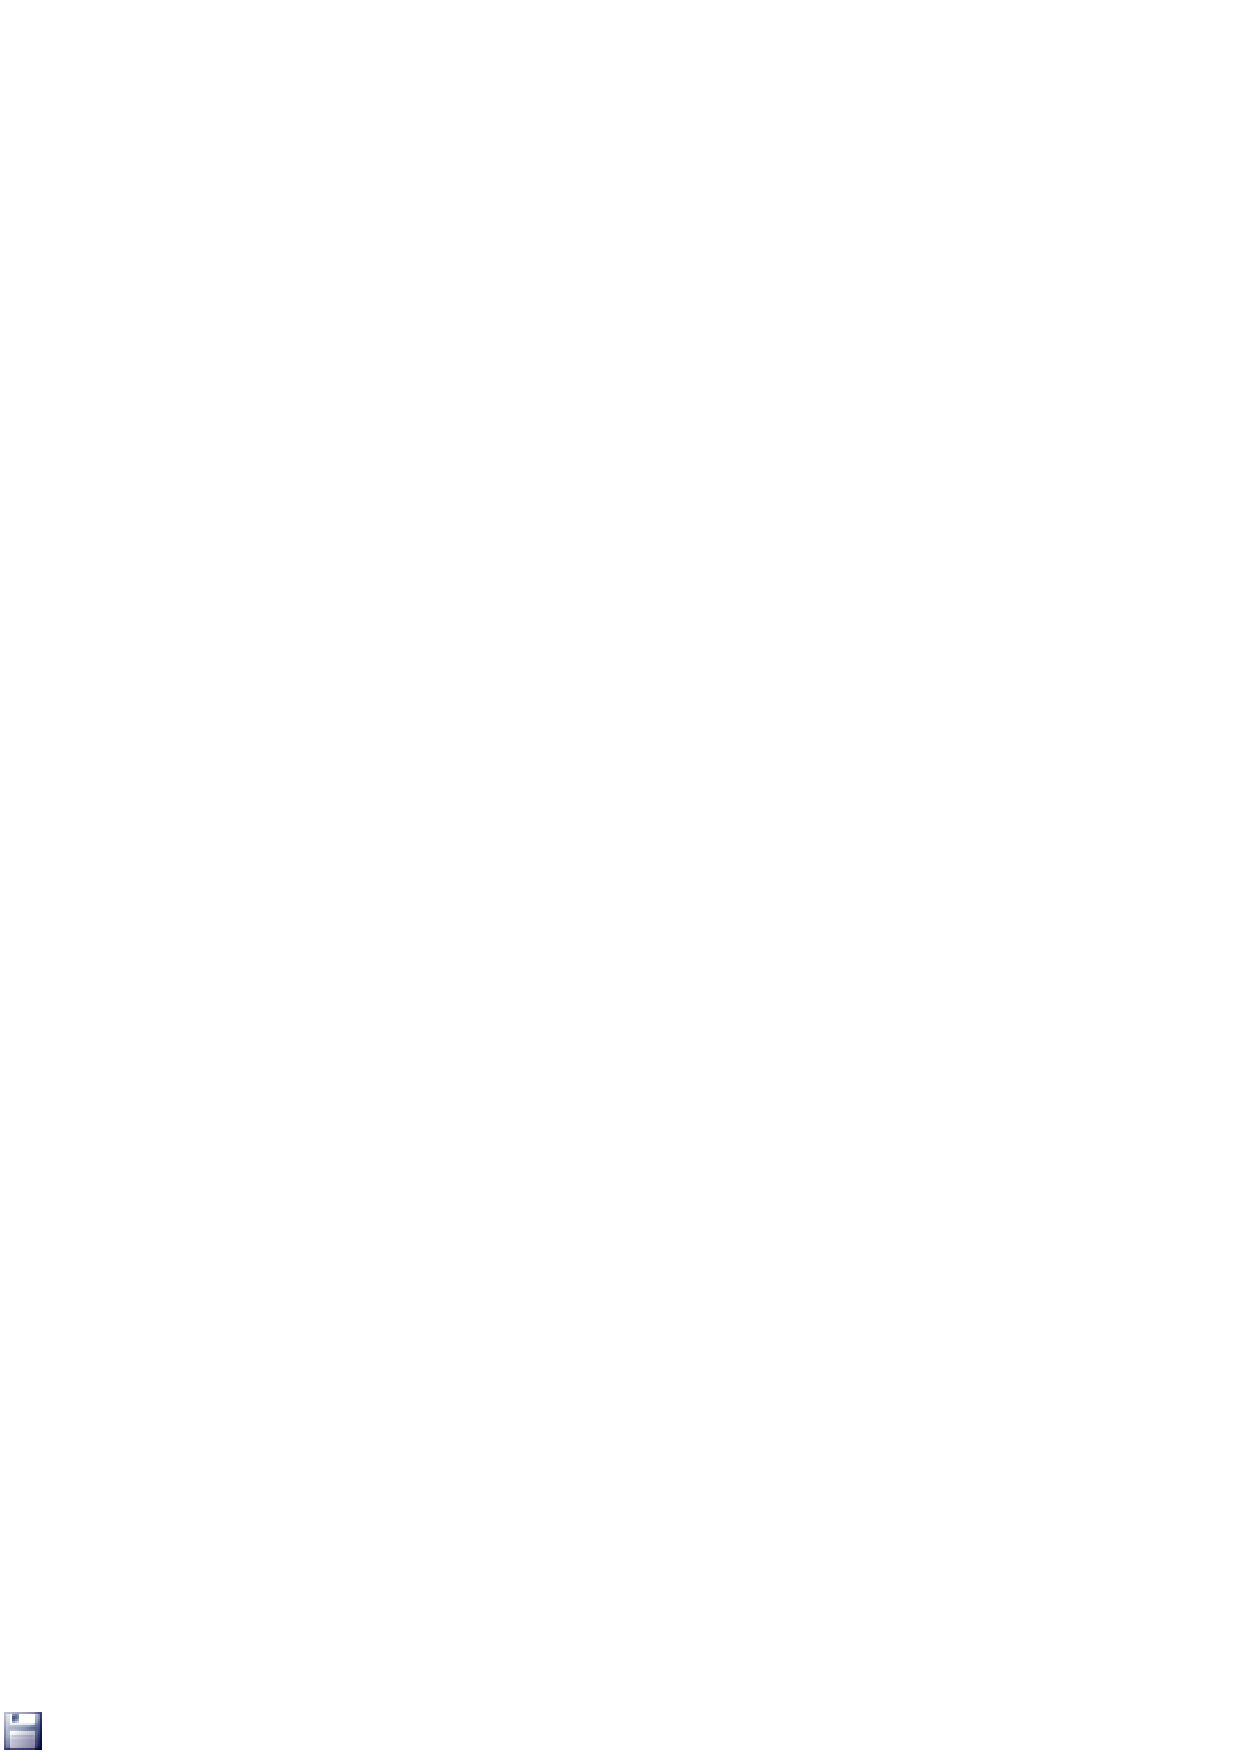
\includegraphics[width=0.7cm]{mActionFileSave}
   & Сохранить изменения
   &  &  \\
\hline
\end{tabular}
\caption{Основные инструменты редактирования векторного слоя}\label{tab:vector_editing}\medskip
\end{table}

Любое редактирование начинается с выбора функции
\dropmenuopttwo{mActionToggleEditing}{Режим редактирования}.
Эта опция доступна из контекстного меню после щелчка правой кнопки мыши
по легенде слоя.\index{Allow Editing}

Также, чтобы начать или закончить редактирование, можно использовать
кнопку \index{Toggle Editing}
\toolbtntwo{mActionToggleEditing}{Режим редактирования} на панели инструментов
по оцифровке.\index{editing!icons} После того, как слой стал редактируемым,
над каждой вершиной появяться специальные маркеры и станут доступны кнопки
с дополнительными функциями из панели инструментов.

\begin{Tip}\caption{\textsc{Регулярное сохранение}}
Не забывайте переключать \toolbtntwo{mActionToggleEditing}{Режим редактирования}
регулярно. Это позволит как сохранить последние изменения, так и удостовериться,
что источники данных могут принять все сделанные изменения.
\end{Tip}

\minisec{Добавление объектов}
\index{vector layers!adding!feature}
\index{vector layers!move!feature}

Можно использовать кнопки на панели инструментов:
\toolbtntwo{mActionCapturePoint}{Создать точку},
\toolbtntwo{mActionCaptureLine}{Создать линию} или
\toolbtntwo{mActionCapturePolygon}{Создать полигон}, чтобы переключить \qg
курсор в режим редактирования.

Для каждого объекта сначала идет оцифровка формы, а затем добавляются атрибуты.
Чтобы начать оцифровку и создать первую точку нового объекта, надо нажать
левой кнопкой мыши по области карты.

Для продолжения линий и полигонов надо продолжать нажимать на левую кнопку
мыши для создания каждого дополнительного узла. Чтобы закончить
редактирование объекта, просто щелкните правой кнопки мыши в любом
месте карты. Это подтверждение того, что редактирование данного объекта
окончено.

В процессе редактирования будет появляться окно атрибутов, позволяя тем
самым вводить информацию для нового объекта.
Рисунок~\ref{fig:vector_digitising} показывает ввод атрибутов для вымышленной реки
Аляски. В вкладке \tab{Оцифровка} из меню \mainmenuopt{Установки} \arrow
\dropmenuopt{Параметры} можно также активировать функцию \\
\checkbox{Не показывать всплывающее окно ввода атрибутов для каждого создаваемого объекта}.

\begin{figure}[ht]
   \centering
   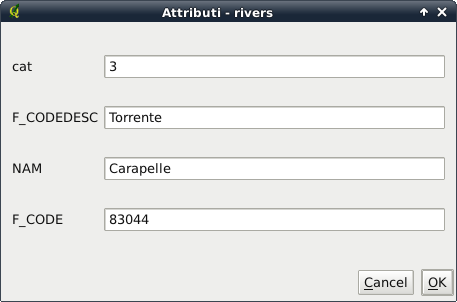
\includegraphics[clip=true, width=8cm]{editDigitizing}
   \caption{Диалог ввода атрибутивных значений после оцифровки нового объекта \nixcaption}\label{fig:vector_digitising}
 \end{figure}

С помощью опции \toolbtntwo{mActionMoveFeature}{Переместить объект} на
панели инструментов можно двигать созданные объекты.

\begin{Tip}\caption{\textsc{Типы значений атрибутов}}
По крайне мере, при редактировании shape-файла типы атрибутов проверяются
во время ввода. Поэтому невозможно ввести числовое значение в текстовое поле
диалога \dialog{Атрибуты} или наоборот. Если это сделать все же необходимо,
то следует отредактировать атрибуты на следующем шаге в диалоге
\dialog{Таблица атрибутов}.
\end{Tip}

\minisec{Редактирование узлов}
\index{vector layers!node!tool}

Как для слоев данных PostgreSQL/PostGIS, так и для слоев, состоящих из
shape-файлов, \\
\toolbtntwo{mActionNodeTool}{Редактирование узлов} предоставляет
возможности изменения узлов объектов, аналогичные имеющимся в программах CAD.
Можно выделить сразу множество вершин и перемещать, добавлять или удалять
их все вместе. Инструмент редактирования узлов работает с включенной функцией
перепроецирования «на лету», а также поддерживает топологическое редактирование
объектов. Этот инструмент, в отличие от остальных инструментов Quantum GIS,
довольно «настойчивый», так, когда некоторая операция выполнена, инструмент
продолжает оставаться активным, а объект выделенным. Если инструмент
редактирования узлов не может обнаружить объекты, на дисплей выдается
предупреждение.

Важно правильно установить \mainmenuopt{Установки} \arrow
\dropmenuopttwo{mActionOptions}{Параметры} \arrow
\tab{Оцифровка} \arrow \selectnumber{{}Радиус поиска}{10}, значение должно быть
больше нуля. В противном случае \qg не распознает редактируемую вершину.

\begin{Tip}\caption{\textsc{Маркировка Вершин}}
Данная версия \qg поддерживает три типа маркировки вершин "--- полупрозрачный
круг, крест и «без маркера». Чтобы изменить стиль маркировки, выберите
\dropmenuopttwo{mActionOptions}{Параметры} из меню \mainmenuopt{Установки}
и на вкладке \tab{Оцифровка} выберите подходящий тип.
\end{Tip}

\minisec{Основные операции}\index{vector layers!Node Tool}

Включите инструмент \toolbtntwo{mActionNodeTool}{Редактирование узлов} и
выделите объект простым нажатием по нему. На месте каждой вершины этого
объекта появится красные рамки. Это основной инструмент выделения объектов.
Его функциональные возможности следующие:

\begin{itemize}[label=--]
\item \textbf{Выделение вершин}: Выделение узла происходит простым нажатием
по нему кнопкой мыши, при этом цвет рамки изменится на синий. Чтобы выделить
несколько узлов одновременно, надо удерживать клавишу
\keystroke{Shift}. Нажатие на
\keystroke{Ctrl} используется для инвертирования выделения узлов (выделенные
узлы становятся невыделенными и наоборот). Также несколько узлов одновременно
можно выделить, если нажать кнопкой мыши где-нибудь в стороне от объекта и
очертить прямоугольную область вокруг интересующего множества вершин. Или
просто нажать на отрезок линии и оба смежных узла будут выделены.
\item \textbf{Добавление узлов}: Добавить узлы также просто. Двойной щелчок
мыши рядом с отрезком линии добавит новую вершину рядом с положением курсора.
Обратите внимание, что вершина появится на ребре объекта, а не точно в
месте курсора,но при необходимости ее можно переместить.
\item \textbf{Удаление узлов}: После выделения вершин для их удаления надо
нажать клавишу \keystroke{Delete}, вершины будут удалены. Обратите внимание,
что согласно стандарту Quantum GIS, необходимое количество узлов для каждого
типа объекта все же останется. Чтобы полностью удалить объект, надо использовать
другой инструмент.
\item \textbf{Перемещение узлов}: Выделите все вершины, которые собираетесь
перемещать. Все выделенные вершины будут перенесены в направлении курсора.
Если активна функция прилипания, все вершины могут перескочить на
ближайшие узлы или линии.
\end{itemize}

При отпускании кнопки мыши, все изменения будут сохранены и появятся в
диалоге отмены. Запомните, что все операции поддерживают топологическое
редактирование, когда оно включено. Перепроецирование «на лету» также
поддерживается.

\minisec{Вырезать, Копировать и Вставить Объекты}
\index{vector layers!cut!feature}
\index{vector layers!copy!feature}
\index{vector layers!paste!feature}
\index{editing!cutting features}
\index{editing!copying features}
\index{editing!pasting features}

Выделенные объекты можно удалять, копировать и вставлять из слоя в слой
одного проекта \qg  при условии, что для них включен
\toolbtntwo{mActionToggleEditing}{Режим редактирования}.

Объекты также можно вставить во внешние приложения в виде текста: объекты
отражаются в формате  CSV, где их геометрия передается форматом
OGC Well-Known Text (WKT).

Однако в настоящей версии  \qg, текстовые объекты из внешних приложений
\qg не могут быть добавлены в слой \qg. Когда же может пригодиться функция
копирования и вставки? Оказывается, возможно редактирование нескольких
слоев одновременно и копирование/вставка объектов между ними. Для чего это
может понадобится? Предположим, необходимо поработать со слоем озер, в
котором интересует только одно или два озера, а не все 5 000, например,
как в нашем слое \filename{big\_lakes}. Тогда можно создать новый слой и,
используя операции копирование/вставка, переместить в него нужные озера.

Рассмотрим пример копирования части озер в новый слой:

\begin{enumerate}
\item Загрузить слой, из которого вы собираетесь копировать (исходный слой)
\item Загрузить или создать слой, в который вы будете копировать (целевой слой)
\item Начать редактирование целевого слоя
\item Активировать исходный слой щелчком мыши по нему в легенде
\item Используя инструмент \toolbtntwo{mActionSelect}{Выбрать объекты},
выделить объект(ы) в исходном слое
\item Выбрать инструмент \toolbtntwo{mActionEditCopy}{Копировать объекты}
\item Сделать активным целевой слой, щелкнув по нему в легенде кнопкой мыши
\item Нажать \toolbtntwo{mActionEditPaste}{Вставить выделенные объекты}
\item Завершить редактирование и сохранить изменения
\end{enumerate}

Что случится, если исходный и целевой слой имеют разную структуру (названия
полей и их типы отличаются)? \qg заполнит совпадающие поля и проигнорирует
остальные. Если результат копирования атрибутов в целевой слой не имеет
значения, то становится неважно, в каком виде они там будут представлены.
Если в целевом слое необходимо сохранить все с точностью "--- объекты и
их атрибуты, необходимо убедиться, что структуры исходного и целевого слоя
совпадают.

\begin{Tip}\caption{\textsc{Соответствие вставляемых объектов}}
Если исходный и целевой слой находятся в одинаковой проекции, тогда
геометрия вставленных объектов будет идентична исходному слою. Однако если
целевой слой находится в отличной проекции, тогда \qg не гарантирует
идентичность геометрии. Это происходит по причине незначительных ошибок
округления, неизбежных при переходе от одной проекции к другой.
\end{Tip}

\minisec{Удаление выделенных объектов}
\index{vector layers!deleting!feature}

Если надо удалить весь полигон, вначале его необходимо выделить, используя
обычный инструмент \\
\toolbtntwo{mActionSelect}{Выбрать объекты}. Также можно
выделить несколько объектов для удаления. После выбора соответствующих
объектов используйте инструмент
\toolbtntwo{mActionDeleteSelected}{Удалить выделенное}, объекты будут удалены.

Инструмент \toolbtntwo{mActionEditCut}{Вырезать выделенные объекты} на панели
инструментов по оцифровке также может использоваться для удаления объектов.
Это действительно удаляет объекты, но также помещает их в «пространственный
буфер». Таким образом, вырезание объектов приводит к их удалению. Затем можно
использовать инструмент \toolbtntwo{mActionEditPaste}{Вставить выделенные объекты},
чтобы вернуть их обратно. Это дает возможность отменить выполненное удаление
объекта. Операции вырезания, копирования и вставки работают только на
выделенных объектах, это означает, что можно работать с несколькими объектами
одновременно.

\begin{Tip}\caption{\textsc{Поддержка удаления объектов}}
Когда редактируется shap-файл ESRI, удаление объектов из него возможно, если
\qg использует версию GDAL 1.3.2 или выше. Версии \qg для операционных
систем OS X и Windows, доступные для скачивания на официальном сайте,
построены с использованием версии GDAL 1.3.2 или выше.
\end{Tip}

\minisec{Сохранение отредактированных слоев}
\index{editing!saving changes}

Когда слой находится в режиме редактирования, любые изменения сохраняются
только в памяти \qg. Поэтому они не сохраняются непосредственно на диск.
Если необходимо сохранить изменения в текущем слое и при этом продолжать
его редактирование, нужно просто нажать на кнопку
\toolbtntwo{mActionFileSave}{Сохранить изменения}. Если выключить режим
редактирования нажав на \toolbtntwo{mActionToggleEditing}{Режим редактирования}
(или просто выйти из \qg), то появится запрос, хотите вы сохранить
изменения или пнет.

Если изменения не могут быть сохранены (например, диск полон или атрибуты
имеют неверное значение), \qg сохранит их в своей памяти. Это позволит
откорректировать изменения и попробовать еще раз.

\begin{Tip}\caption{\textsc{Целостность данных}}
Создание резервной копии данных перед началом редактирования "--- это
всегда хорошая идея. Несмотря на то, что авторы \qg сделали все возможное
для сохранения ваших данных, они по-прежнему не дают никаких гарантий в
этом отношении.
\end{Tip}

\subsection{Дополнительные функции оцифровки}
\index{vector layers!advanced digitizing}
\index{advanced digitizing!an existing layer}
\label{sec:advanced_edit}

\begin{table}[h]\index{vector layers!advanced editing tools}
\centering
\small
\begin{tabular}{|l|p{6.9cm}|l|p{6.9cm}|}
\hline \textbf{Иконка} & \textbf{Назначение} & \textbf{Иконка} & \textbf{Назначение} \\
\hline 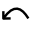
\includegraphics[width=0.7cm]{mActionUndo}
   & Отменить
   & 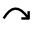
\includegraphics[width=0.7cm]{mActionRedo}
   & Вернуть \\
\hline \includegraphics[width=0.7cm]{mActionSimplify}
   & Упростить объект
   & \includegraphics[width=0.7cm]{mActionAddRing}
   & Добавить кольцо \\
\hline \includegraphics[width=0.7cm]{mActionAddIsland}
   & Добавить часть
   & \includegraphics[width=0.7cm]{mActionDeleteRing}
   & Удалить кольцо \\
\hline \includegraphics[width=0.7cm]{mActionDeletePart}
   & Удалить часть
   & \includegraphics[width=0.7cm]{mActionReshape}
   & Корректировать объекты \\
\hline \includegraphics[width=0.7cm]{mActionSplitFeatures}
   & Разбить объекты
   & \includegraphics[width=0.7cm]{mActionMergeFeatures}
   & Объединить выбранные объекты \\
\hline \includegraphics[width=0.7cm]{mActionRotatePointSymbols}
   & Повернуть значки
   &
   & \\
\hline
\end{tabular}
\caption{Дополнительные возможности редактирования векторного слоя}\label{tab:advanced_editing}
\end{table}

\minisec{Отменить и Вернуть}
\index{vector layers!undo}
\index{vector layers!redo}

Инструменты \toolbtntwo{mActionUndo}{Отменить} и
\toolbtntwo{mActionRedo}{Вернуть} позволяют отменить либо вернуть
последний или какой-то конкретный шаг при редактировании векторных данных.
Основной вид операций Отменить/Вернуть представляет из себя виджет, где
показаны все действия (см. Рисунок~\ref{fig:vector_redoundo}). Этот виджет
по умолчанию не показывается, чтобы он появился, надо нажать правой кнопкой
мыши по панели инструментов и кликнуть по флажку Отменить/Вернуть. Однако
функция Отменить/Вернуть активна, даже если виджет не выведен на экран.

При нажатии кнопки Отменить состояние всех объектов и их атрибутов
возвращается на шаг назад. Изменения, произведенные в каком-либо другом
месте (например, в одном из модулей), могут иметь неспецифические названия
для своих операций, которые появляются в этой закладке. Операции можно
отменить или оставить их изменения.

Действия можно отменить простым нажатием на кнопки Отменить или Вернуть,
либо выбрать непосредствено на пункт из списка, который хотите отменить.
Другая возможность отменить операцию "--- нажать на кнопку
\button{Отменить/Вернуть} на панели инструментов дополнительных возможностей
редактирования.

\begin{figure}[ht]
   \centering
   \includegraphics[clip=true, width=12cm]{redo_undo}
   \caption{Отмена и Возврат операций редактирования \nixcaption}\label{fig:vector_redoundo}
\end{figure}

\minisec{Упростить объект}
\index{vector layers!simplify}

Инструмент \toolbtntwo{mActionSimplify}{Упростить объект} позволяет уменьшить
количество вершин объекта, при том, что геометрия объекта не изменяется.
Необходимо выделить объект, после чего он будет подсвечен красным и появится
ползунок. Двигая ползунок, красная опоясывающая линия менят свою форму,
показывая тем самым, как объект будет упрощен.Если нажать кнопку \button{OK}
новая упрощенная геометрия будет сохранена. Если объект не может быть
упрощен (например, мультиполигоны), появится всплывающее окно предупреждения.

\minisec{Добавить кольцо}
\index{vector layers!add!ring}

Можно создать кольцевой полигон, используя функцию
\toolbtntwo{mActionAddRing}{Добавить кольцо} на панели инструментов. Внутри
существующего полигона можно оцифровать последующий полигон, который
превратиться в <<отверстие>>, таким образом, только оставшаяся область
между границами внешнего и внутреннего полигона и будет кольцевым полигоном.

\minisec{Добавить часть}
\index{vector layers!add!part}

Можно использовать \toolbtntwo{mActionAddIsland}{Добавить часть}
для добавления новых полигонов к мультиполигональным объектам. Новая
полигональная часть должна быть создана за границами мультиполигона.


\minisec{Удалить кольцо}
\index{vector layers!delete!ring}

Инструмент \toolbtntwo{mActionDeleteRing}{Удалить кольцо} позволяет удалять
кольцевые полигоны внутри существующей площади. Этот инструмент работает
только с полигональными слоями. Никакик изменений не произойдет, если
инструмент применяется на внешнем контуре полигона. Инструмент может
применяться как для полигональных объектов, так и на мультиполигональных.
Перед тем, как выделить вершины кольца, настройте порог прилипания для вершин.


\minisec{Удалить часть}
\index{vector layers!delete!part}

Инструмент \toolbtntwo{mActionDeletePart}{Удалить часть} позволяет удалять
части мультиполигональных объектов (например, удалить полигон
мультиполигонального объекта). Инструмент не сможет удалить последнюю часть
объекта. Она останется нетронутой. Инструмент работает со всеми типами
геометрии: точками, линиями, полигонами. Перед тем, как выделить вершины
части, необходимо настроить порог прилипания для вершин.

\minisec{Корректировать объекты}
\index{vector layers!reshape!feature}

Можно корректировать форму линий и полигонов, используя инструмент
\toolbtntwo{mActionReshape}{Корректировать объекты}, расположенный на
панели инструментов. Он удаляет часть линии или полигона между первым и
последним пересечением с исходной линией. При работе с полигонами это
может иногда привести к непредсказуемым результатам. Этот инструмент
наиболее пригоден для корректировки небольших частей полигонов. Редактирование
нескольких  полигональных объектов одновременно невозможно, так как при этом
будут создаваться полигоны с ошибочной геометрией.

\textbf{Примечание}: Инструмент корректировки объектов может изменять начало
кольца полигона или замкнутой линии. Так, точка, представленная тут «дважды»
больше не будет таковой. Это не должно быть проблемой при использовании
большинства приложений, но, тем не менее, это необходимо иметь ввиду.

\minisec{Разбивка объектов}
\index{vector layers!split!feature}

Можно разбить объекты, используя инструмент
\toolbtntwo{mActionSplitFeatures}{Разбить объекты} на панели
инструментов. Чтобы разбить объект, просто нарисуйте линию через него.

\minisec{Объединить выделенные объекты}
\index{vector layers!merge!features}

Инструмент \toolbtntwo{mActionMergeFeatures}{объединить выделенные объекты}
позволяет объединять объекты, которые имеют общие границы и атрибуты.

\minisec{Повернуть значки}
\index{vector layers!rotate!symbol}

Инструмент \toolbtntwo{mActionRotatePointSymbols}{Повернуть значки} позволяет
изменить поворот точечного символа на карте, если задано вращение по столбцу
атрибутивной таблицы точечного слоя на вкладке \tab{Символика} из меню
свойств слоя "--- \dialog{Свойства}. В другом случае инструмент будет не
активен.

\begin{figure}[ht]
   \centering
   \includegraphics[clip=true, width=6cm]{rotatepointsymbol}
   \caption{Поворот точечного символа \nixcaption}\label{fig:rotatepoint}
\end{figure}

Чтобы повернуть объект, выделите точечный объект на карте и вращайте его,
удерживая нажатой левую кнопку мыши. При этом будет отображаться красная
стрелка с величиной угла поворота (см. Рисунок~\ref{fig:rotatepoint}).
Когда вы отпустите левую кнопку мыши,в таблице атрибутов обновится значение.

\textbf{Примечание}: Если удерживать кнопку \keystroke{Ctrl} нажатой, поворот
будет осуществляться с шагом 15 градусов.

\subsection{Создание новых shape-слоев и слоев Spatialite}\label{sec:create shape}\index{editing!creating a new
shape layer}

\qg позволяет создавать новые shape-слои и слои Spatialite. Создание новых
слоев GRASS осуществляется с помощью модуля GRASS. Для более подробной
информации по созданию слоев GRASS обратитесь к Разделу~\ref{sec:creating_new_grass_vectors}.

\minisec{Создание нового  shape-слоя}\label{sec:create shape}\index{editing!creating a new shapefile layer}

Чтобы создать новый редактируемый shape-файл, выберите \button{Создать} \arrow
\toolbtntwo{mActionNewVectorLayer}{Создать новый shape-файл} из меню
\mainmenuopt{Слой}. Появится диалог \dialog{Новый векторный слой}, как показано
на Рисунке~\ref{fig:newvectorlayer}. Выберите тип слоя (точка, линия или полигон).

\begin{figure}[ht]
   \centering
   \includegraphics[clip=true, width=8cm]{editNewVector}
   \caption{Диалог создания нового shape-файла \nixcaption}\label{fig:newvectorlayer}
\end{figure}

Обратите внимание, что \qg пока еще не поддерживает создание объектов в
размерности 2.5D (т.\,е. объектов с координатами X, Y, Z), кроме того, не
поддерживается создание объектов с линейной системой координат (координата M).
В настоящее время можно создавать только shape-файлы. В будущих
версиях \qg будет поддерживаться создание любых слоев типов OGR или PostgreSQL.

В завершении создания shape-файла следует добавить желаемые атрибуты. Для
этого надо нажать на кнопку  \button{Добавить} и задать имя и тип атрибутов.
Поддерживаются только следующие типы атрибутов:  \selectstring{{}Тип}{Текст},
\selectstring{{}Тип}{Целое число}, и \selectstring{{}Тип}{Десятичное число}.
Дополнительно, в соответствии с выбранным типом атрибута, можно определить
размер и точность для нового поля атрибутов. Как только все необходимые
параметры заданы, нажмите кнопку \button{OK} и задайте имя для выходного
shape-файла. \qg автоматически добавит к имени файла расширение \filename{.shp}.
После того, как shape-файл создан, он будет добавлен в карту и доступен для
обычного редактирования, как описано в Разделе~\ref{sec:edit_existing_layer} выше.

\minisec{Создание нового слоя SpatiaLite}\label{sec:create spatialite}\index{editing!creating a new spatialite layer}

Чтобы создать новый редактируемый слой SpatiaLite, выберите \button{Создать}
\arrow \toolbtntwo{mActionNewVectorLayer}{Создать слой SpatiaLite} из меню
\mainmenuopt{Слой}. Появится диалог \dialog{Создать слой SpatiaLite}, как
показано на Рисунке~\ref{fig:newspatialitelayer}.

\begin{figure}[ht]
   \centering
   \includegraphics[clip=true, width=8cm]{editNewSpatialite}
   \caption{Диалоговое окно Создать слой SpatiaLite \nixcaption}\label{fig:newspatialitelayer}
\end{figure}

Первый шаг "--- выбрать существующую базу данных Spatialite или создать
новую. Загрузить существующую базу данных можно нажав на кнопку \button{...}
справа от поля имени для базы данных. Затем следует задать имя новому слою и
определить тип слоя и EPSG SRID. По желанию можно выбрать \\
\checkbox{создать первичный ключ с автоматическим приращением}.

Чтобы задать таблицу атрибутов для нового слоя Spatialite, добавьте имена
и определите соответствующие типы данных для новых столбцов таблицы, затем
нажмите кнопку \button{Добавить}. В завершении нажмите кнопку \button{OK}.
\qg автоматически добавит новый слой в легенду, и он будет доступен для
обычного редактирования, как описано в Разделе~\ref{sec:edit_existing_layer} выше.

В диалоговом окне по созданию spatialite слоя можно создать несколько слоев,
нажимая на кнопку \button{Apply}, при этом нет необходимости закрывать
диалоговое окно.

\subsection{Работа с таблицей атрибутов}
\label{sec:attribute table}
\index{editing!working with the attribute table}

Таблица атрибутов представляет объекты выделенного слоя. Каждая строка таблицы
соответствует одному объекту на карте и отражает его атрибуты в столбцах.
Объекты в таблице можно искать, выделять, перемещать и редактировать.

Чтобы открыть таблицу атрибутов векторного слоя, необходимо сделать его активным,
нажав по нему кнопкой мыши в легенде карты. Затем в меню \mainmenuopt{Слой}
выберите \dropmenuopttwo{mActionOpenTable}{Открыть таблицу атрибутов}.
Также можно открыть таблицу атрибутов, щелкнув по слою в легенде правой
кнопкой мыши, и выбрав \\
\dropmenuopttwo{mActionOpenTable}{Открыть таблицу атрибутов}
из выпадающего меню. Откроется новое окно, в котором будут представлены атрибуты
для каждого объекта слоя (cм. Рисунок~\ref{fig:attributetable}). Количество
объектов указано в заголовке атрибутивной таблицы.

\begin{figure}[ht]
   \centering
   \includegraphics[clip=true, width=12cm]{vectorAttributeTable}
   \caption{Attribute Table for Alaska layer \nixcaption}\label{fig:attributetable}
\end{figure}

\minisec{Выделение объектов по таблице атрибутов}

\textbf{Выделенная строка} в таблице атрибутов представляет все атрибуты
выделенного объекта слоя. Таблица атрибутов отражает все изменения в
выделении объектов слоя через главное окно карты или наоборот. Смена
выделения в таблице атрибутов приводит к изменению выделения в главном
окне карты, также выделение другого объекта слоя приводит к выделению
соответствующей ему строки таблицы.

Строки можно выделить, если нажать кнопкой мыши на номер строки, расположеный
с левой стороны от нее. Выделение строки не меняет текущего положения курсора.
\textbf{Несколько строк} можно выделить, удерживая клавишу \keystroke{Ctrl}.
\textbf{Сквозное выделение} может также применяться, для этого необходимо
удерживать клавишу \keystroke{Shift} и выбрать несколько строк, также
нажимая на их номера-заголовки, расположенных слева. Все строки между
текущим положением курсора и выбранными строками будут выделены.

Каждый столбец может быть отсортирован. Для этого надо нажать кнопкой мыши
по его заголовку. Небольшая стрелка отражает порядок сортировки (направленная
вниз стрелка означает убывание величины от верхних строк к нижним,
направленная вверх стрелка означает увеличение величины от верхних строк
к нижним ).

Для \textbf{простого поиска по атрибутам} только по одному столбцу можно
использовать поле \button{Искать?}. Выберите поле (столбец), по которому
хотите произвести поиск, из выпадающего меню и нажмите кнопку \button{Поиск}.
Количество сопоставленных записей появится в окне результатов. Для более
сложного поиска используйте Расширенный поиск \button{...}, который будет
описан в Разделе~\ref{sec:select_by_query}.

Чтобы отобразить только выбранные строки, нажмите кнопкой мыши в окошке \\
\checkbox{Показать только выбранные записи}. Для поиска только по выделенным
записям активируйте \\
\checkbox{Искать только в выбранных записях}. Остальные
кнопки, расположенные слева снизу атрибутивной таблицы, обладают следующими
функциональными возможностями:

\begin{itemize}[label=--]
\item \toolbtntwo{mActionOpenTable}{Снять выделение}
\item \toolbtntwo{mActionSelectedToTop}{Переместить выделенные в начало}
\item \toolbtntwo{mActionInvertSelection}{Обратить выделение}
\item \toolbtntwo{mActionCopySelected}{Копировать выбранные строки в буфер обмена}
также с \keystroke{Ctrl-C}
\item \toolbtntwo{mActionZoomToSelected}{Увеличить карту до выбранных строк}
также с \keystroke{Ctrl-J}
\item \toolbtntwo{mActionToggleEditing}{Режим редактирования} для
редактирования отдельных значений таблицы атрибутов и активации функций,
описанных ниже.
\item \toolbtntwo{mActionDeleteSelected}{Удалить выделенные объекты}
\item \toolbtntwo{mActionNewAttribute}{Добавить поле} для слоев PostGIS
и OGR с версией GDAL >= 1.6.
\item \toolbtntwo{mActionDeleteAttribute}{Удалить поле} пока только для
слоев PostGIS.
\item \toolbtntwo{mActionCalculateField}{Открыть калькулятор полей}
\end{itemize}

\begin{Tip}\caption{\textsc{Управление атрибутивными данными}}
В настоящее время только для слоев PostGIS поддерживается добавление или
удаление столбцов атрибутов с помощью этого диалогового окна. В
будущих версиях \qg другие источники данных также будут поддерживаться,
так как это нововведение было недавно добавлено в GDAL/OGR > 1.6.0
\end{Tip}

\section{Query Builder}\label{sec:query_builder}
\index{Query Builder}

The \button{Advanced search\dots} button opens the Query Builder and allows you to
define a subset of a table using a SQL-like WHERE clause, display the result in the
main window and save it as a Shapefile. For example, if you have a
\filename{towns} layer
with a \usertext{population} field you could select only larger towns by entering
\usertext{population > 100000} in the SQL box of the query builder. Figure
\ref{fig:query_builder} shows an example of the query builder populated with
data from a PostGIS layer with attributes stored in PostgreSQL.
The Fields, Values and Operators sections help the user to construct the SQL-like
WHERE clause easily in the text field SQL where clause window.


\begin{figure}[ht]
  \centering
    \includegraphics[clip=true, width=11.5cm]{queryBuilder}
    \caption{Query Builder \nixcaption}\label{fig:query_builder}
\end{figure}

The \textbf{Fields list} contains all attributes of the attribute table to be
searched. To add an attribute to the SQL where clause field, double click its
name in the Fields list. Generally you can use the various fields, values and
operators to construct the query or you can just type it into the SQL box.

The \textbf{Values list} lists the values of an attribute. To list all possible
values of an attribute, select the attribute in the Fields list and click the
\button{All} button\index{Query Builder!getting all values}. To list all values
of an attribute that are present in the sample table, select the attribute in
the Fields list and click the \button{Sample}
button\index{Query Builder!generating sample list}. To add a value to the SQL
where clause field, double click its name in the Values list.

The \textbf{Operators section} contains all usable operators. To add an operator
to the SQL where clause field, click the appropriate button. Relational operators
( = , > , \dots), string comparison operator ( LIKE ), logical operators ( AND , OR
, \dots) are available.

The \button{Clear} button clears the text in the SQL where clause text field. The
\button{Test} button shows a message box with the number of features satisfying
the current query, which is usable in the process of query construction. The
\button{OK} button closes the window and selects the features satisfying the
query. The \button{Cancel} button closes the window without changing the current
selection.

\begin{Tip}\caption{\textsc{Changing the Layer Definition}}\index{Query
Builder!changing layer definitions}
You can change the layer definition after it is loaded by altering
the SQL query used to define the layer. To do this, open the
vector \dialog{Layer Properties} dialog by double-clicking on the layer in the legend and click on the
\button{Query Builder} button on the \tab{General} tab. See Section
\ref{sec:vectorprops} for more information.
\end{Tip}

\minisec{Select by query}\label{sec:select_by_query}

With \qg it is possible also to select features using a similar query builder
interface to that used in \ref{sec:query_builder}. In the above section
the purpose of the query builder is to only show features meeting the
filter criteria as a 'virtual layer' / subset. The purpose of the select by
query function is to highlight all features that meet a particular criteria.
Select by query can be used with all vector data providers.

To do a `select by query' on a loaded layer, click on the
button \toolbtntwo{mActionOpenTable}{Open Table} to open the attribute table of the layer. Then
click the \button{Advanced...} button at the bottom. This starts the Query Builder
that allows to define a subset of a table and display it as described in Section
\ref{sec:query_builder}.

\section{Field Calculator}\label{sec:field_calculator}
\index{PostgreSQL!field calculator}
\index{PostGIS!field calculator}
\index{OGR!field calculator}
\index{field calculator!PostgreSQL}
\index{field calculator!PostGIS}
\index{field calculator!OGR}

The \toolbtntwo{mActionCalculateField}{Field Calculator} button in the
attribute table allows to perform calculations on basis of existing
attribute values or defined functions, e.g to calculate length or area
of geometry features. The results can be written to a new attribute column
or it can be used to update values in an already existing column. The creation
of new attribute fields is currently only possible in PostGIS and with OGR
formats, if GDAL version is >= 1.6.0.

You have to bring the vector layer in editing mode, before you can click on
the field calculator icon to open the dialog (see Figure
\ref{fig:field_calculator}). In the dialog you first have to select, whether
you want to update an existing field, only update selected features or
create a new attribute field, where the results of the calculation will be added.

\begin{figure}[ht]
  \centering
    \includegraphics[clip=true, width=11.5cm]{fieldcalculator}
    \caption{Field Calculator \nixcaption}\label{fig:field_calculator}
\end{figure}

If you choose to add a new field, you need to enter a field name, a field type
(integer, real or string), the total field width, and the field precision.
For example, if you choose a field width of 10 and a field precision of 3 it
means you have 6 signs before the dot, then the dot and another 3 signs for the
precision.

The \textbf{Fields list} contains all attributes of the attribute table to be
searched. To add an attribute to the Field calculator expression field, double
click its name in the Fields list. Generally you can use the various fields,
values and operators to construct the calculation expression or you can just
type it into the box.

The \textbf{Values list} lists the values of an attribute field. To list all
possible values, select the attribute field in the Fields list and click the
\button{All} button\index{Field Calculator!getting all values}. To list all
values of an attribute field that are present in the sample table, select the
attribute in the Fields list and click the \button{Sample} button\index{Field
Calcultor!generating sample list}. The procedure is the same as for the Query
Builder. To add a value to the Field calculator expression box, double click its
name in the Values list.

The \textbf{Operators section} contains all usable operators. To add an operator
to the Field calculator expression box, click the appropriate button. Mathematical
calculations ( + , - , * \dots), trigonometric functions ( sin, cos, tan, \dots),
extract geometric information ( length and area ) are available and will be
extended in future versions.

A short example illustrates how the field calculator works. We want to calculate
the length of the 'railroads' layer from the \filename{\qg\_example\_dataset}:

\begin{enumerate}
\item Load the Shapefile \filename{railroads.shp} in \qg and open
the \dialog{Attribute Table} dialog.
\item Click on \toolbtntwo{mActionToggleEditing}{Toggle editing mode} and
open the \toolbtntwo{mActionCalculateField}{Field Calculator} dialog.
\item Unselect the \checkbox{Update existing field} checkbox to enable the
new field box.
\item Add 'length' as output field name, 'real' as output field type and define
output field width 10 and a precision of 3.
\item Now click on Operator 'length' to add it as \$length into the
field calculator expression box and click \button{Ok}.
\end{enumerate}
